%%%%%%%%%%%%%%%%%%%%%%%%%%%%%%%%%%%%%%%%%
% Beamer Presentation
% LaTeX Template
% Version 1.0 (10/11/12)
%
% This template has been downloaded from:
% http://www.LaTeXTemplates.com
%
% License:
% CC BY-NC-SA 3.0 (http://creativecommons.org/licenses/by-nc-sa/3.0/)
%
%%%%%%%%%%%%%%%%%%%%%%%%%%%%%%%%%%%%%%%%%

%----------------------------------------------------------------------------------------
%	PACKAGES AND THEMES
%----------------------------------------------------------------------------------------

\documentclass[aspectratio=169, hyperref={colorlinks=true,pdfpagelabels=false,linkcolor=black}, xcolor=dvipsnames,10pt]{beamer}
\hypersetup{pdftex=true, colorlinks=true, breaklinks=true, linkcolor=black, menucolor=blue, pagecolor=blue, urlcolor=cyan}


\usepackage{graphicx} % Allows including images
\usepackage{booktabs} % Allows the use of \toprule, \midrule and \bottomrule in tables
\usepackage{xcolor, color}% ,colortbl}
\usepackage{tikz} % nalipour
\usetikzlibrary{tikzmark} % nalipour
\usepackage{hyperref}
\usetikzlibrary{shapes,arrows, decorations.pathreplacing} %nilou
\usetikzlibrary{decorations.markings} %nilou
\usetikzlibrary{trees}%nilou
\usetikzlibrary{decorations.pathmorphing}%nilou 
\usepackage{siunitx}%nilou
\usepackage{framed}%nilou
\usetikzlibrary{backgrounds} %nilou
\usepackage[framemethod=tikz]{mdframed}%nilou
\usepackage{adjustbox} %nilou for adjusting the table
\usepackage{amssymb} %nalipour for checkmark
\usepackage{libertine} % For the font

%\usepackage{../../../CLICdp_definitions} % nalipour
\usepackage{xspace}
\usepackage{upgreek} % nalipour
\usepackage{amsmath, mathtools} % nalipour
\renewcommand{\thefootnote}{\fnsymbol{footnote}} % nalipour: symbols
                                % for the footnote
\usepackage{verbatim} % nalipour
\usepackage{fixltx2e}
\usepackage{adjustbox}%nalipour
\usepackage{pifont} %nalipour
\usepackage{smartdiagram}
\usesmartdiagramlibrary{additions}
\usepackage{siunitx}

\usetikzlibrary{angles,quotes}
\usetikzlibrary{positioning}

%%%%%%%%%%%%%%%%%%%%%%%%%%%%%

%----------------------------------------------------------------------------------------
%	TITLE PAGE
%----------------------------------------------------------------------------------------
\title[]{
Simulation of the drift chamber for the FCCee-IDEA detector concept within FCCSW}
\author[Niloufar Alipour Tehrani]{Niloufar Alipour Tehrani
  \vspace{0.3cm} }

\institute[CERN]{} 
\date[12 April 2018]{Common detector technology: \\ \vspace{0.1cm}
	Common software\\ \vspace{0.5cm}
  \scriptsize{FCC Week 2018 \\ Amsterdam, the Netherlands \\ \vspace{0.3cm}
12 April 2018}}


\setbeamertemplate{navigation symbols}{}
\setbeamertemplate{footline}[frame number]

\usetheme{default}%CambridgeUS}%Boadilla}%Pittsburgh}
\usecolortheme{default}

\setlength{\leftmargini}{2pt} % nalipour: left margin indentation
\renewcommand{\inserttotalframenumber}{\ref{lastframe}} 
\begin{document}
\renewcommand{\inserttotalframenumber}{\pageref{lastslide}}

\tikzset{cross/.style={cross out, draw=black, minimum
    size=2*(#1-\pgflinewidth), inner sep=0pt, outer sep=0pt}, %default
  radius will be 1pt.  cross/.default={1pt}}


%%%%%%%%%%%%%%%%%%%%%%%%%%%%%
%         SLIDE             %
%%%%%%%%%%%%%%%%%%%%%%%%%%%%%
\begin{frame}[plain]
  
  \vspace{1cm}
  
  \titlepage

  \vspace{-1.5cm}
  \begin{columns}
    \column{0.25\textwidth}
    \centering
    
\includegraphics[width=\textwidth]{../logos/FCC-logo}
    \column{0.5\textwidth}
    \column{0.25\textwidth}
    \centering
    
\includegraphics[width=0.6\textwidth]{../logos/logo_cern.pdf}
  \end{columns}
\end{frame}



%%%%%%%%%%%%%%%%%%%%%%%%%%%%%
%         SLIDE             %
%%%%%%%%%%%%%%%%%%%%%%%%%%%%%
\begin{frame}
	\frametitle{FCC Software: FCCSW}
	
	\begin{columns}
	\column{0.5\textwidth}
	\begin{itemize}
	\item Common software for all FCC experiments
		\begin{itemize}
		\item ee, hh \& eh \vspace{0.5cm}
		\end{itemize}
	\item Detector and physics studies
		\begin{itemize}
		\item Fast \& full simulations
		\item One software stack from event generation to
                  physics analysis \vspace{0.5cm}
		\end{itemize}
	\item Collaborative approach
		\begin{itemize}
		\item LHC: Gaudi
		\item CLIC: DD4hep
		\item New solutions $\Rightarrow$ where needed
		\end{itemize}
	\end{itemize}
	
	\column{0.5\textwidth}
	\centering
	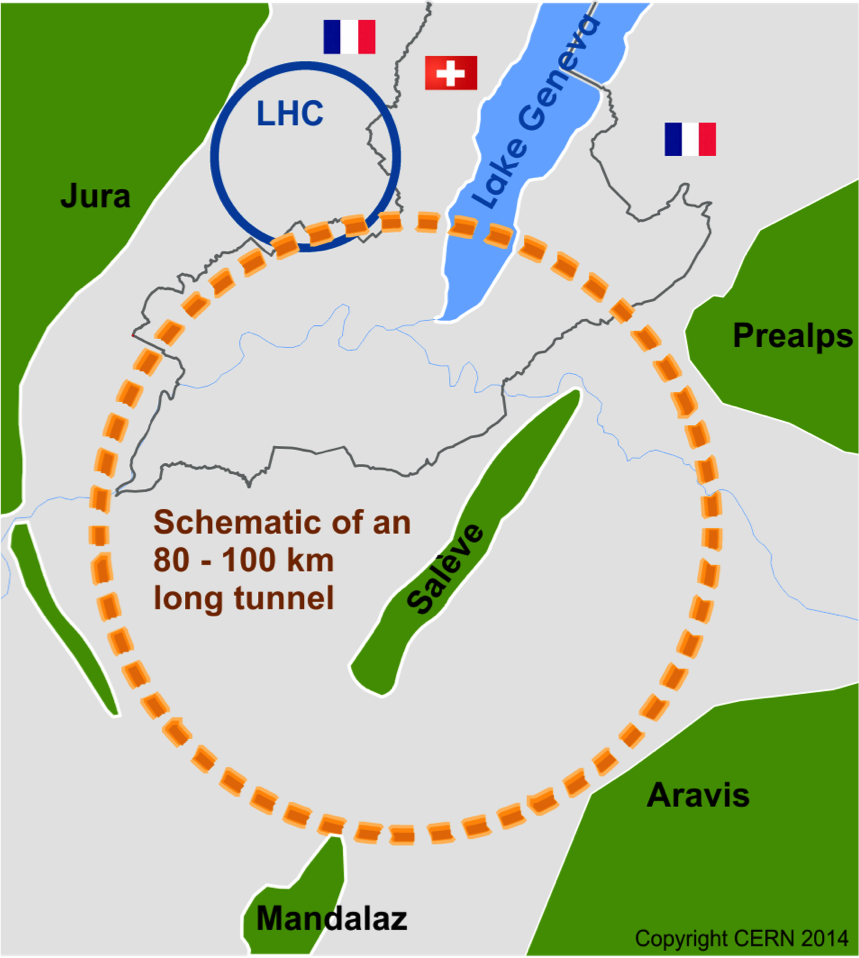
\includegraphics[width=\textwidth]{../figures/cernFCC}
	\end{columns}
	

\end{frame}

%%%%%%%%%%%%%%%%%%%%%%%%%%%%%
%         SLIDE             %
%%%%%%%%%%%%%%%%%%%%%%%%%%%%%
\begin{frame}
	\frametitle{2 FCCee detector concepts}
	
		\begin{itemize}
		\item The CLD detector concept (c.f. CLD detector model overview, Oleksandr~Viazlo)
			\begin{itemize}
			\item An adaptation of the CLIC detector model 
			\\ $\Rightarrow$ (Silicon-based vertex and tracking detectors)
			\item Widely simulated with the ILCSoft
			\end{itemize}
		\item The IDEA detector concept $\Rightarrow$ \textcolor{Red}{focus of this talk}
			\begin{itemize}
			\item Simulated using FCCSW
			\end{itemize}
		\end{itemize}

	
	\begin{columns}
	\column{0.5\textwidth}
	
	\begin{block}{IDEA: Ultimate Goal}
	\begin{itemize}
	\item Vertex detector: MAPS
	\item Ultra-light drift chamber with PID (DCH)
	\item Double read-out calorimetry (DR)
        \item Additional disk layers to be placed in the space between DCH and DR 
	\item 2~T solenoidal magnetic field
	\item Instrumented return yoke
	\item Surrounded by large tracking volume (R$\sim$8~m) for very weakly coupled (long-lived) particles
	\end{itemize}
	\end{block}

	\column{0.5\textwidth}
        \vspace{-1cm}
	\centering
	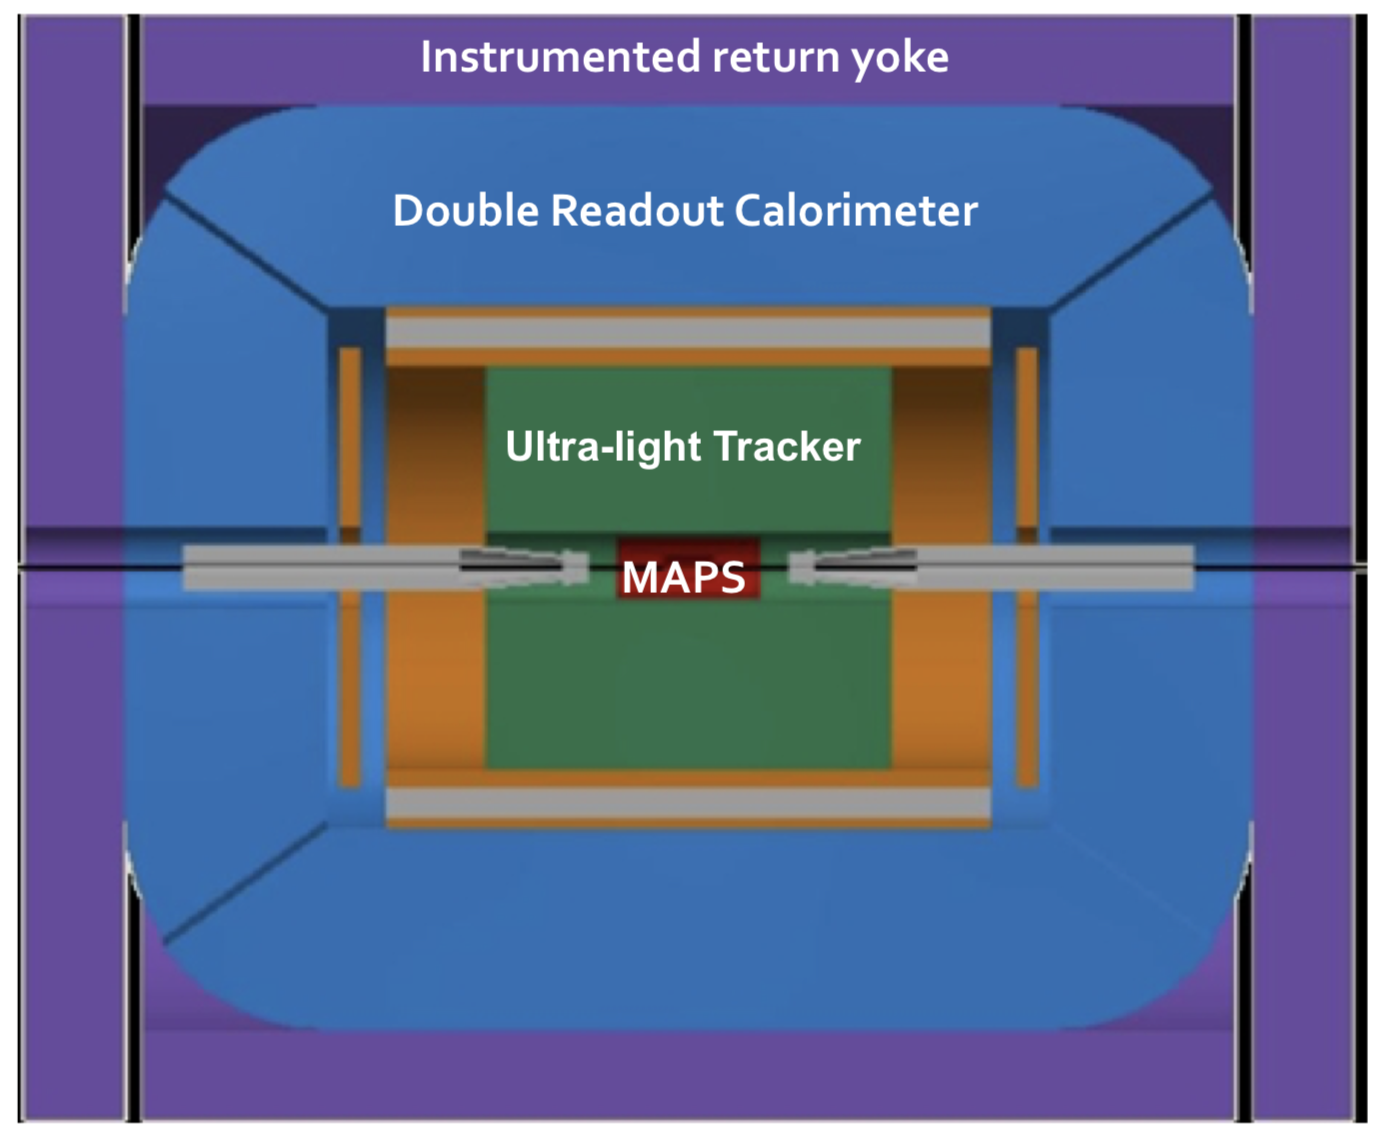
\includegraphics[width=\textwidth]{../figures/FCCeeIDEAConcept.png}
	\end{columns}

\end{frame}

%%%%%%%%%%%%%%%%%%%%%%%%%%%%%
%         SLIDE             %
%%%%%%%%%%%%%%%%%%%%%%%%%%%%%
\begin{frame}
	\frametitle{IDEA Drift Chamber (DCH)}
	
	\begin{columns}	
	\column{0.5\textwidth}
	
	\begin{itemize}
	\item Track reconstruction \& particle ID
	\item Layers divided into cells rotated with a certain stereo angle
	\end{itemize}


	\begin{block}{Parameters}
  	\begin{table}
    	\begin{adjustbox}{max width=\textwidth}
    	  \begin{tabular}{l l}
    	    \toprule
        % & Dimensions    \\
        % \hline
        Length & 4500 mm \\ 
        Inner radius & 345 mm \\
        Outer radius & 2000 mm\\
        Nb. layers & 112 \\
        Cell size & 12 mm to 14.7~mm\\
        Total nb. of sensitive wires & 56448 \\
        Total nb. of field wires & 282240 \\
        Total nb. of wires & 338688 \\
        Gas & GasHe\_90Isob\_10 \\
        Wire material & Aluminum \\
        Single cell resolution & 0.1 mm \\
        \bottomrule
      \end{tabular}
    	\end{adjustbox}
  	\end{table}
	\end{block}


	\column{0.5\textwidth}
	
	\begin{itemize}
	\item Field wires: provide a uniform electric field
	\item Sensitive wires: record signal
	\item Field to sense wire ratio: 5:1
	\end{itemize}
	
	
	\centering
	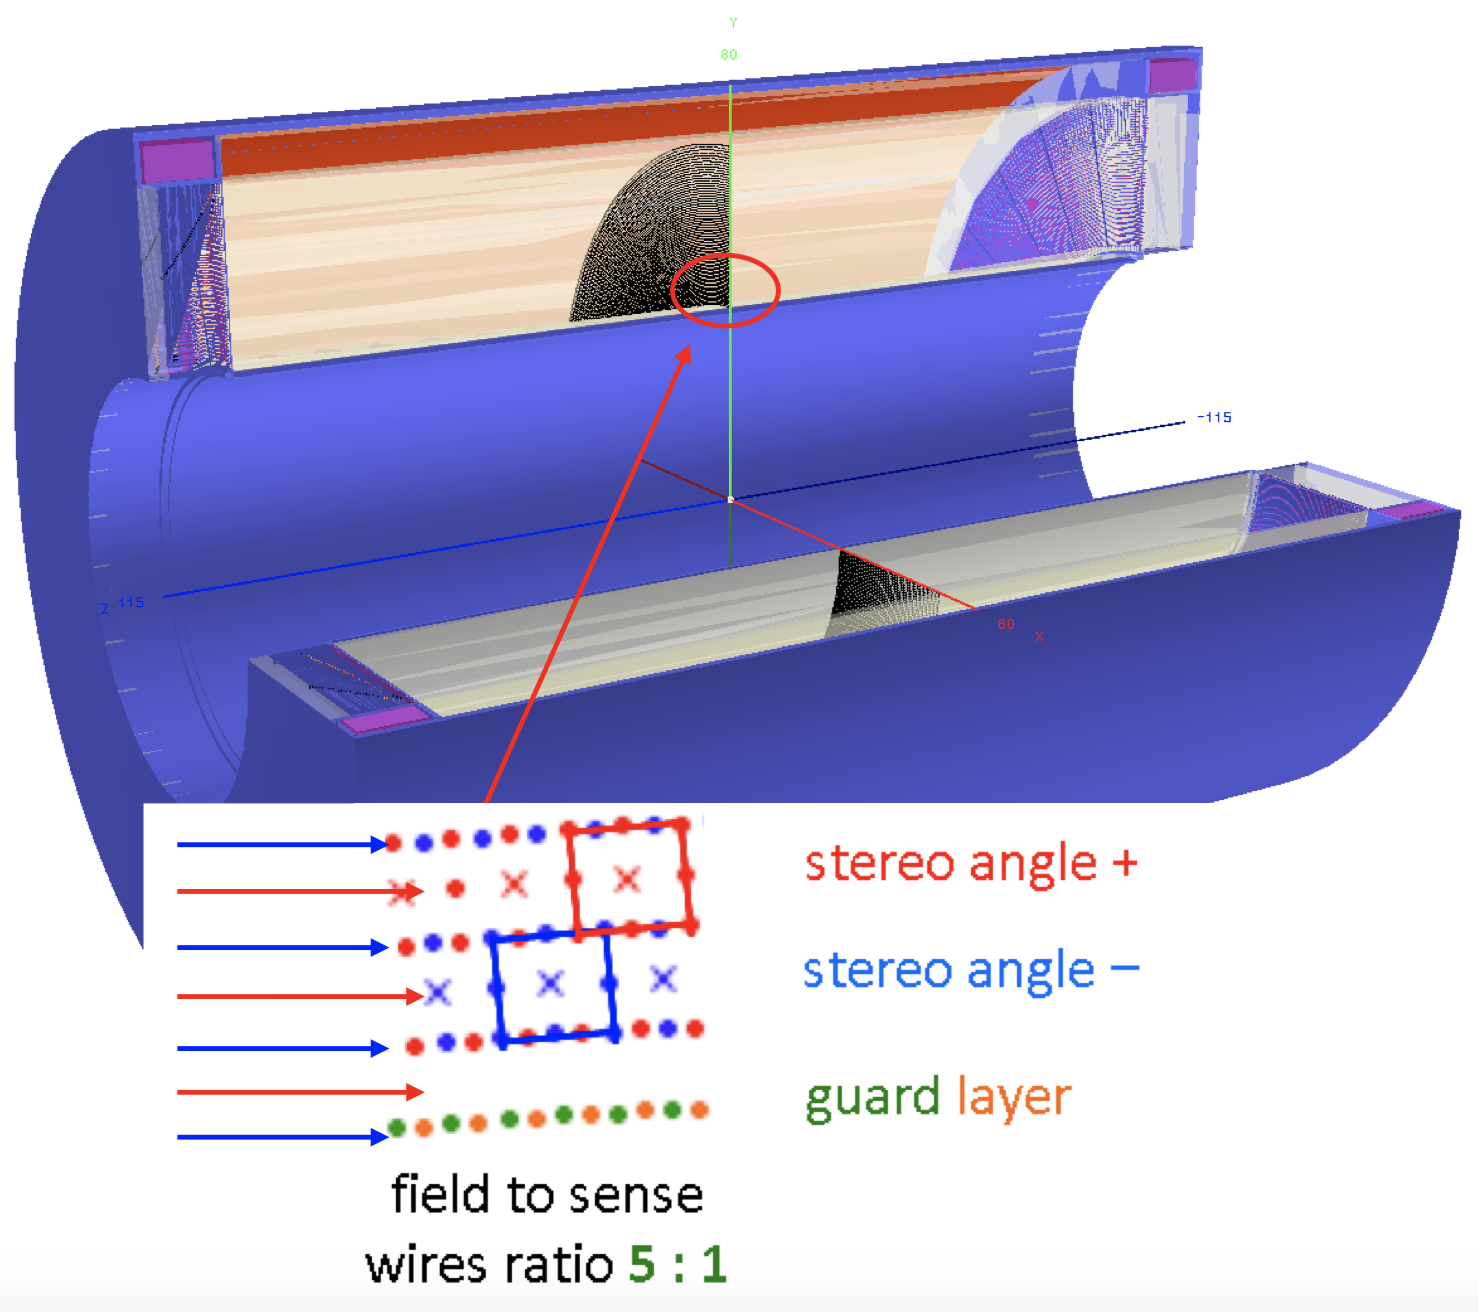
\includegraphics[width=\textwidth]{../figures/DriftChamber.png}
	\end{columns}
\end{frame}



%%%%%%%%%%%%%%%%%%%%%%%%%%%%%
%         SLIDE             %
%%%%%%%%%%%%%%%%%%%%%%%%%%%%%
\begin{frame}
	\frametitle{FCCSW simulation chain}
	
	\begin{enumerate}
	\item Detector geometry description with DD4hep
		\begin{itemize}
		\item Collaborative effort with CLIC, ILC and LHCb
		\item The IR region and the VXD from CLD are as well implemented in DD4hep
		\item Definition of the gas layers in the DCH 
		\end{itemize}
	\item Segmentation of the sensitive areas:
		\begin{itemize}
		\item Information on the position of the sense wires instead of placing physical volumes
		\item Speed up the simulation
		\end{itemize}
	\item Geant4 simulation:
		\begin{itemize}
		\item Calculate the E\textsubscript{dep} for each ionisation action
		\item Charge drift to the wires
		\end{itemize}
	\item Hit reconstruction:
		\begin{itemize}
		\item Combination of individual hit calculations from (3)
		\item Calculation of the signal in the wire
		\end{itemize}
	\end{enumerate}		
	
        \centering
	\smartdiagramset{back arrow disabled=true}
  	\smartdiagram[flow diagram:horizontal]
  	{%
    	{Geometry\\DDhep}, Segmentation, {Geant4 \\simulation}, Hit Reconstruction%
  	}
  	

\end{frame}

%%%%%%%%%%%%%%%%%%%%%%%%%%%%%
%         SLIDE             %
%%%%%%%%%%%%%%%%%%%%%%%%%%%%%
\begin{frame}
	\frametitle{1. Geometry}
	
	\begin{itemize}
	\item Beam-pipe and interaction region (IR) taken from the CLD concept.
	\item Vertex detector also taken from the CLD concept.
	\item The drift chamber implemented from scratch in FCCSW.
	\end{itemize}
	
	\begin{block}{Visualisation with FCCSW}
	\centering
	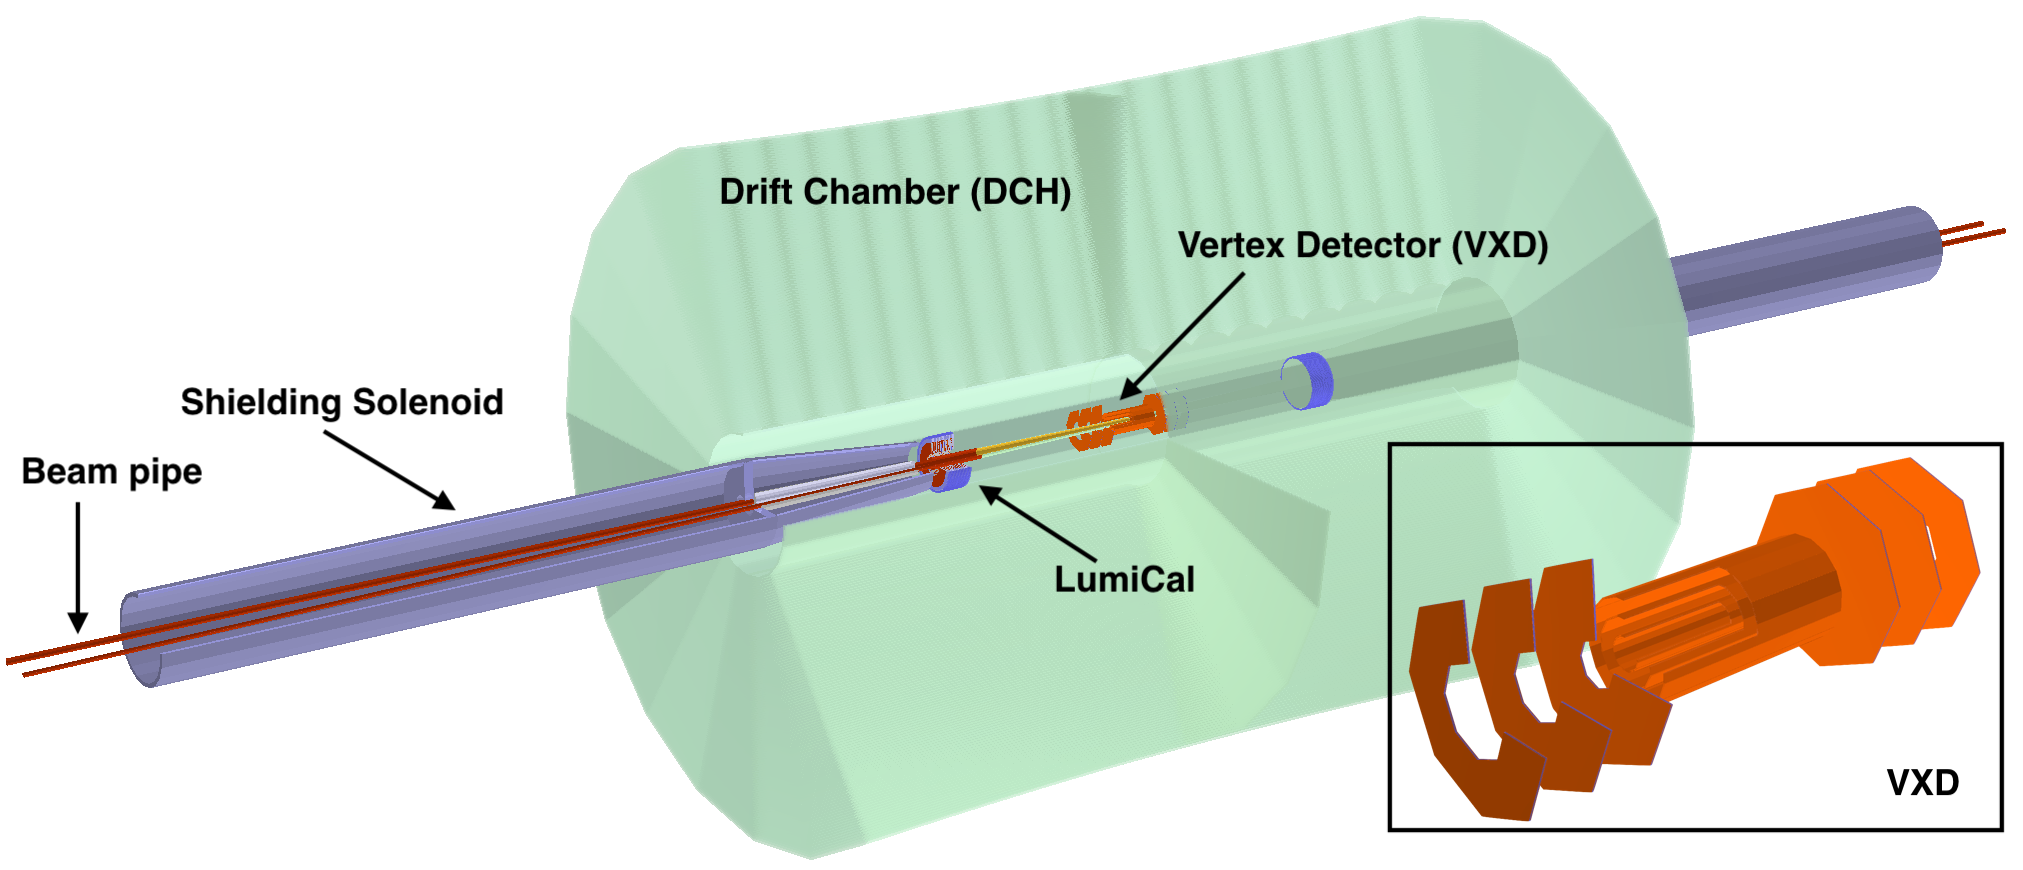
\includegraphics[width=\textwidth]{../figures/FCCeeIDEA_IR_description_zoomVXD.png}
	\end{block}

\end{frame}



%%%%%%%%%%%%%%%%%%%%%%%%%%%%%
%         SLIDE             %
%%%%%%%%%%%%%%%%%%%%%%%%%%%%%

\begin{frame}
  \frametitle{2. Segmentation Strategy for DCH (1)}


    \begin{itemize}
    \item Large number of wires $\Rightarrow$ requires a fast way to find the
      location of the closest wire hit
    \item Compute the azimuth angle of the hit $\phi$ for $(x_{hit},
      y_{hit})$ 
      \begin{itemize}
      \item (like if the wires were parallel to the z-axis).
      \end{itemize}

    \begin{equation}
      \phi = \arctan(y_{hit}/x_{hit})
    \end{equation}

    \item The angle between the hit position and the wire detecting it
      is calculated:

    \begin{equation}
      \alpha = 2 \arcsin({{z_{hit} tan(\epsilon)} \over {2R}})
    \end{equation}
  \item Total hit azimuthal angle: $\phi+\alpha$
    \end{itemize}


    \begin{columns}
      \column{0.33\textwidth}
      \column{0.33\textwidth}
      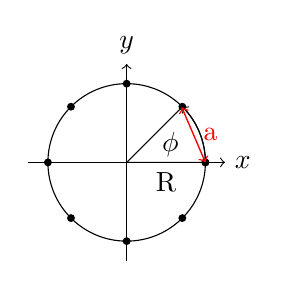
\begin{tikzpicture}[scale=0.5]

        \pgfmathsetmacro{\R}{2}
        \pgfmathsetmacro{\wireAng}{45}
        
        \coordinate (O) at (0,0);
        \foreach \angle in 
        {0,45,...,360} 
        { 
          \fill (\angle:\R) circle (0.1cm); 
        } 
        \draw (0,0) circle (\R);

        \draw 
        (\R,0) coordinate (xcoord) -- 
        node[midway,below] {R} (O) -- 
        (\wireAng:\R) coordinate (slcoord)
        pic [draw,->,angle radius=1cm,"$\phi$"] {angle = xcoord--O--slcoord};

        \draw[<->,line width=0.5pt,red] (\R, 0) -- (1.4, 1.4) node
        (deltay) [midway,right] {a};

        \begin{scope}[]
          \draw[->] (-2.5,0) -- (2.5,0) node[right] {$x$};
          \draw[->] (0,-2.5) -- (0,2.5) node[above] {$y$};
        \end{scope}
      \end{tikzpicture}

      \column{0.33\textwidth}
    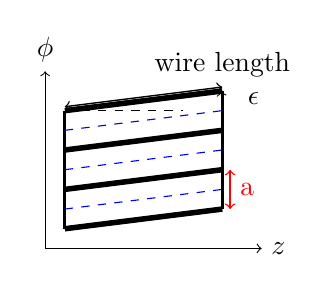
\begin{tikzpicture}[scale=0.5]
      \begin{scope}
        \coordinate (origin) at (0,4);

        \draw[->] (-0.5,0.5) -- (5,0.5) node[right] {$z$};
        \draw[->] (-0.5, 0.5) -- (-0.5,5) node[above] {$\phi$};

        \draw[-,line width=1pt] (0, 1) -- (0, 4);
        \draw[-,line width=1pt] (4, 1.5) -- (4, 4.5);

        \draw[-,line width=2pt] (0, 1) -- (4, 1.5);
        \draw[-,line width=2pt] (0, 2) -- (4, 2.5);
        \draw[-,line width=2pt] (0, 3) -- (4, 3.5);
        \draw[-,line width=2pt] (0, 4) -- (4, 4.5) node
        (pivot) [] {};
        \draw[<->,line width=0.5pt] (0, 4.1) -- (4, 4.6) node
        (length) [above] {wire length};
        \draw[<->,line width=0.5pt,red] (4.2, 1.5) -- (4.2, 2.5) node
        (deltay) [midway, right] {a};

        \draw[-,dashed, line width=0.5pt] (origin) -- (3, 4) node
        (horizon) [] {};
        \pic [draw, ->, "$\epsilon$", angle eccentricity=1.2, angle radius=2cm] {angle = horizon--origin--pivot};


        \draw[-,dashed, blue] (0, 1.5) -- (4, 2);
        \draw[-, dashed, blue] (0, 2.5) -- (4, 3);
        \draw[-, dashed, blue] (0, 3.5) -- (4, 4);

        % \draw[-,blue,line width=1pt] (2, 5) -- (2, 0.7) node
        % (segz) [right] {z segmentation (w)};
      \end{scope}
    \end{tikzpicture}
    \end{columns}


\end{frame}

%%%%%%%%%%%%%%%%%%%%%%%%%%%%%
%         SLIDE             %
%%%%%%%%%%%%%%%%%%%%%%%%%%%%%
\begin{frame}
	\frametitle{2. Segmentation: validation in simulation (2)}
		
	\begin{columns}[t]
		\column{0.5\textwidth}
		\begin{itemize}
		\item Information on the location of the sensitive wires \vspace{0.2cm}
		\item Associates a unique wire ID (cellID) to the wires \vspace{0.2cm}ß
		\item Different granularity for different layers in the DCH \vspace{0.2cm}
		\item The segmentation information is created while building geometry \vspace{0.2cm} \\
			$\Rightarrow$ Accessible in every step of the simulation
		\end{itemize}
	
		\column{0.5\textwidth}	
		\begin{itemize}
		\item First layer of the DCH
		\item Hits having the same wire ID are shown by the same color
		\item Validates the segmentation
		\end{itemize}
		\centering
		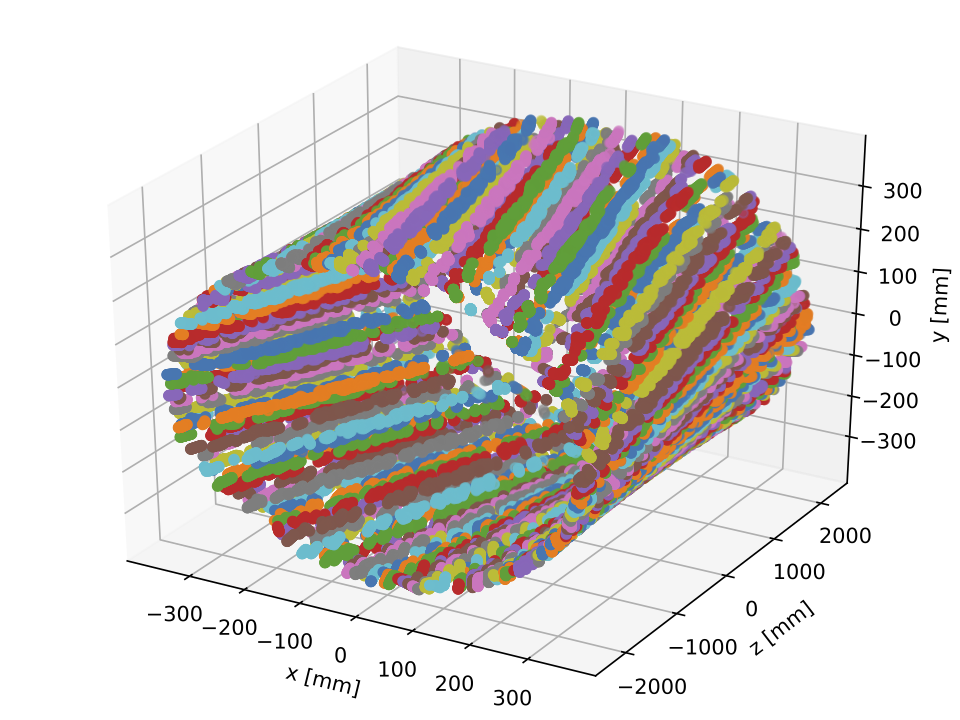
\includegraphics[width=\textwidth]{../figures/allHits}
	\end{columns}
	
\end{frame}

%%%%%%%%%%%%%%%%%%%%%%%%%%%%%
%         SLIDE             %
%%%%%%%%%%%%%%%%%%%%%%%%%%%%%
\begin{frame}
	\frametitle{3. Hit simulation and reconstruction of the DCH }
	
	\begin{block}{Hit Simulation}
	\begin{itemize}
	\item Geant4: Stepping in the gas with a G4Step length of 2~mm 
	\item Reject ionisation acts with:
		\begin{itemize}
		\item E\textsubscript{dep}$<$~10~eV
		\item \texttt{G4Step} length~$<~5\mu$m
		\end{itemize} 
	
	\item Drift the charge deposition to the nearest wire 
		\begin{itemize}
		\item Compute the distance of the closest approach
		\item Calculate the drift time assuming a constant drift velocity of 2~cm/$\mu$s
		\item Smear with the timing resolution of ????
		\item Calculate the total time of the hit \\
		\begin{equation}
	      t_{hit} = t_{drift}+t_{\text{signal}}+t_{\text{particle flight}}
    		\end{equation}
		\end{itemize} 
	\end{itemize}
	\end{block}
		
	\begin{block}{Reconstruction}
		\begin{itemize}
		\item \textcolor{Red}{Hit}: regroup the E\textsubscript{dep} with a drift time smaller than the maximum drift time in the cell
		\end{itemize}
	\end{block}

	
	
\end{frame}


%%%%%%%%%%%%%%%%%%%%%%%%%%%%%
%         SLIDE             %
%%%%%%%%%%%%%%%%%%%%%%%%%%%%%
\begin{frame}
	\frametitle{Number of sensitive layers vs. $\theta$}
	
	\begin{itemize}
		\item Number of layers hit by 100~GeV $\mu-$ 
		\begin{itemize}

		\item $\theta=0^{\circ}$: in the forward direction
		\item $\theta=90^{\circ}$: in the barrel
		\item Averaged over $\phi$	
		\end{itemize}
	\end{itemize}
		
	\begin{columns}	
		\column{0.5\textwidth}	
		\begin{block}{VXD}
		\centering
		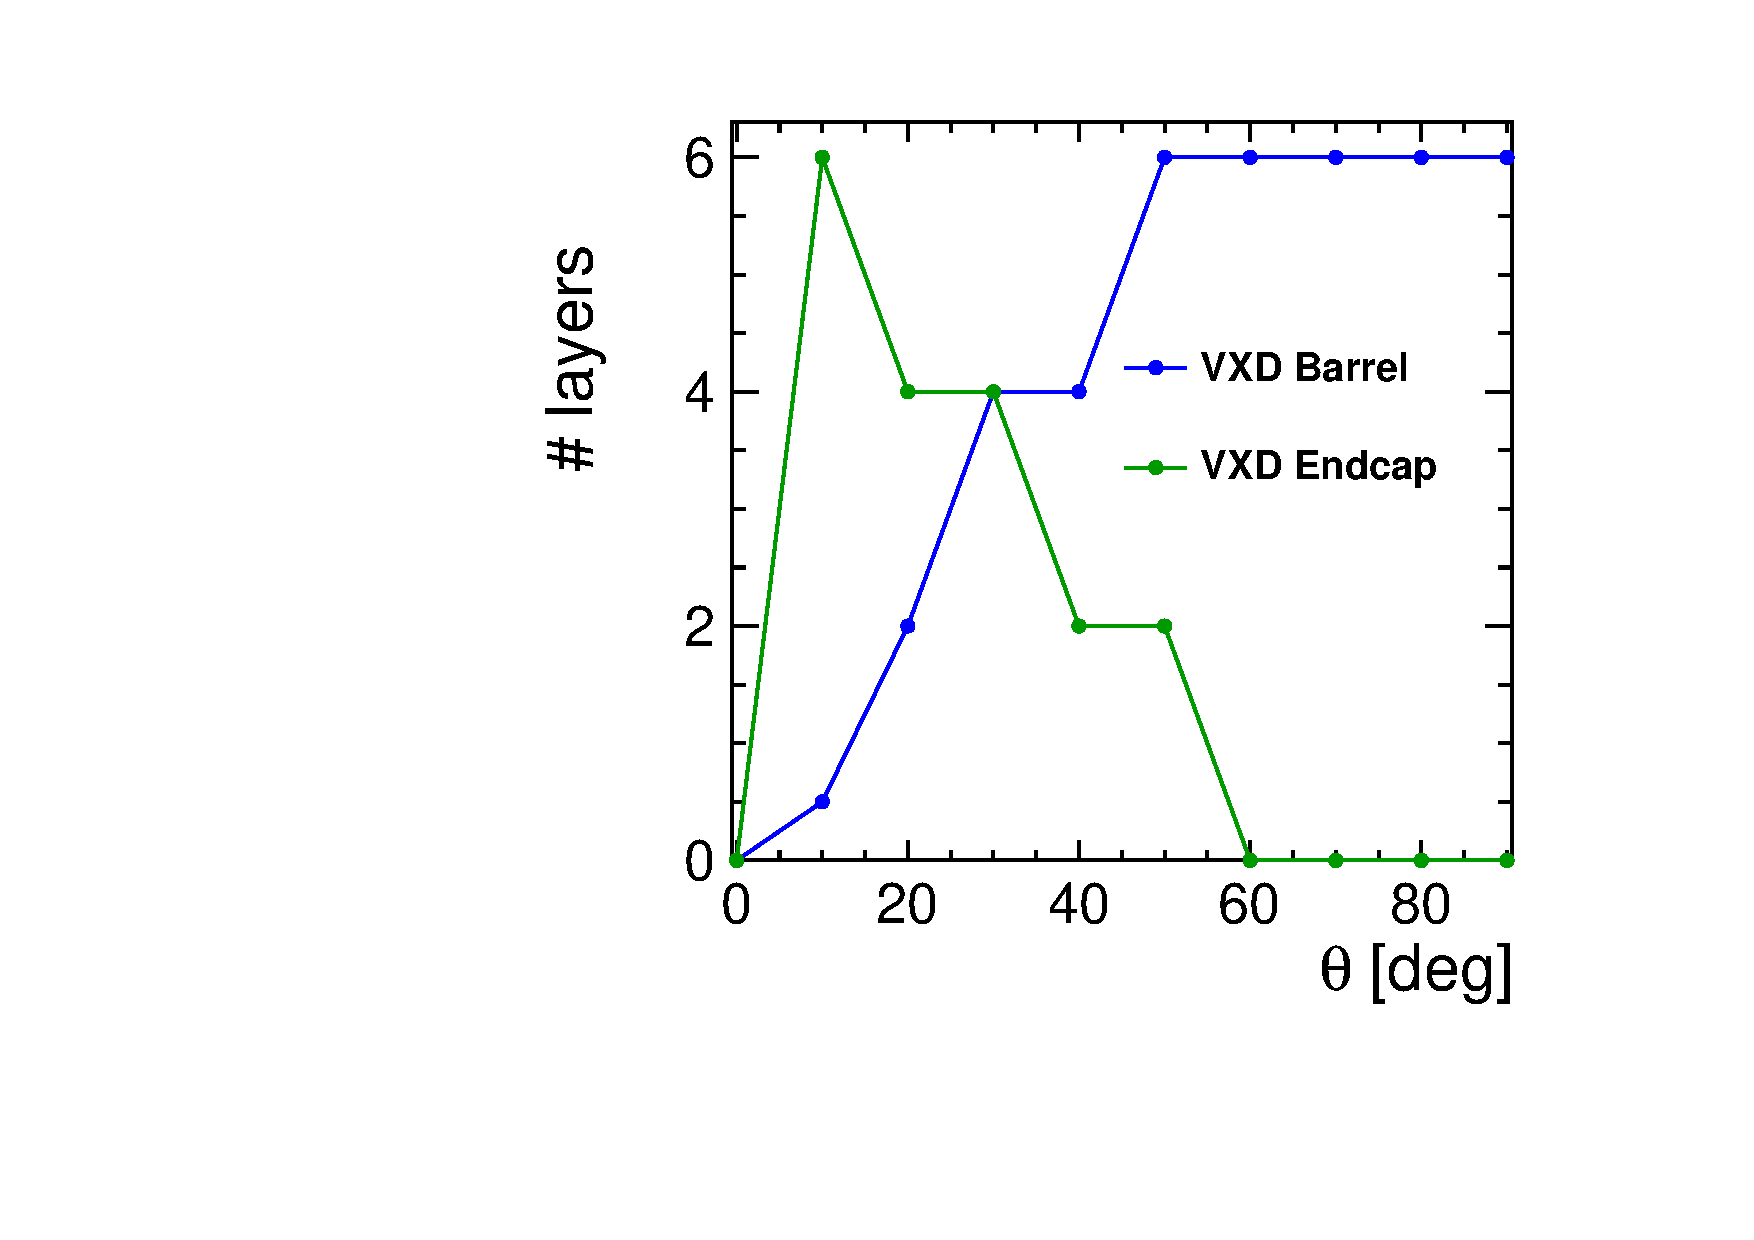
\includegraphics[width=\textwidth]{../figures/theta_nbHits_VXD.pdf}
		\end{block}
	
		\column{0.5\textwidth}	
		\begin{block}{DCH}
		\centering
		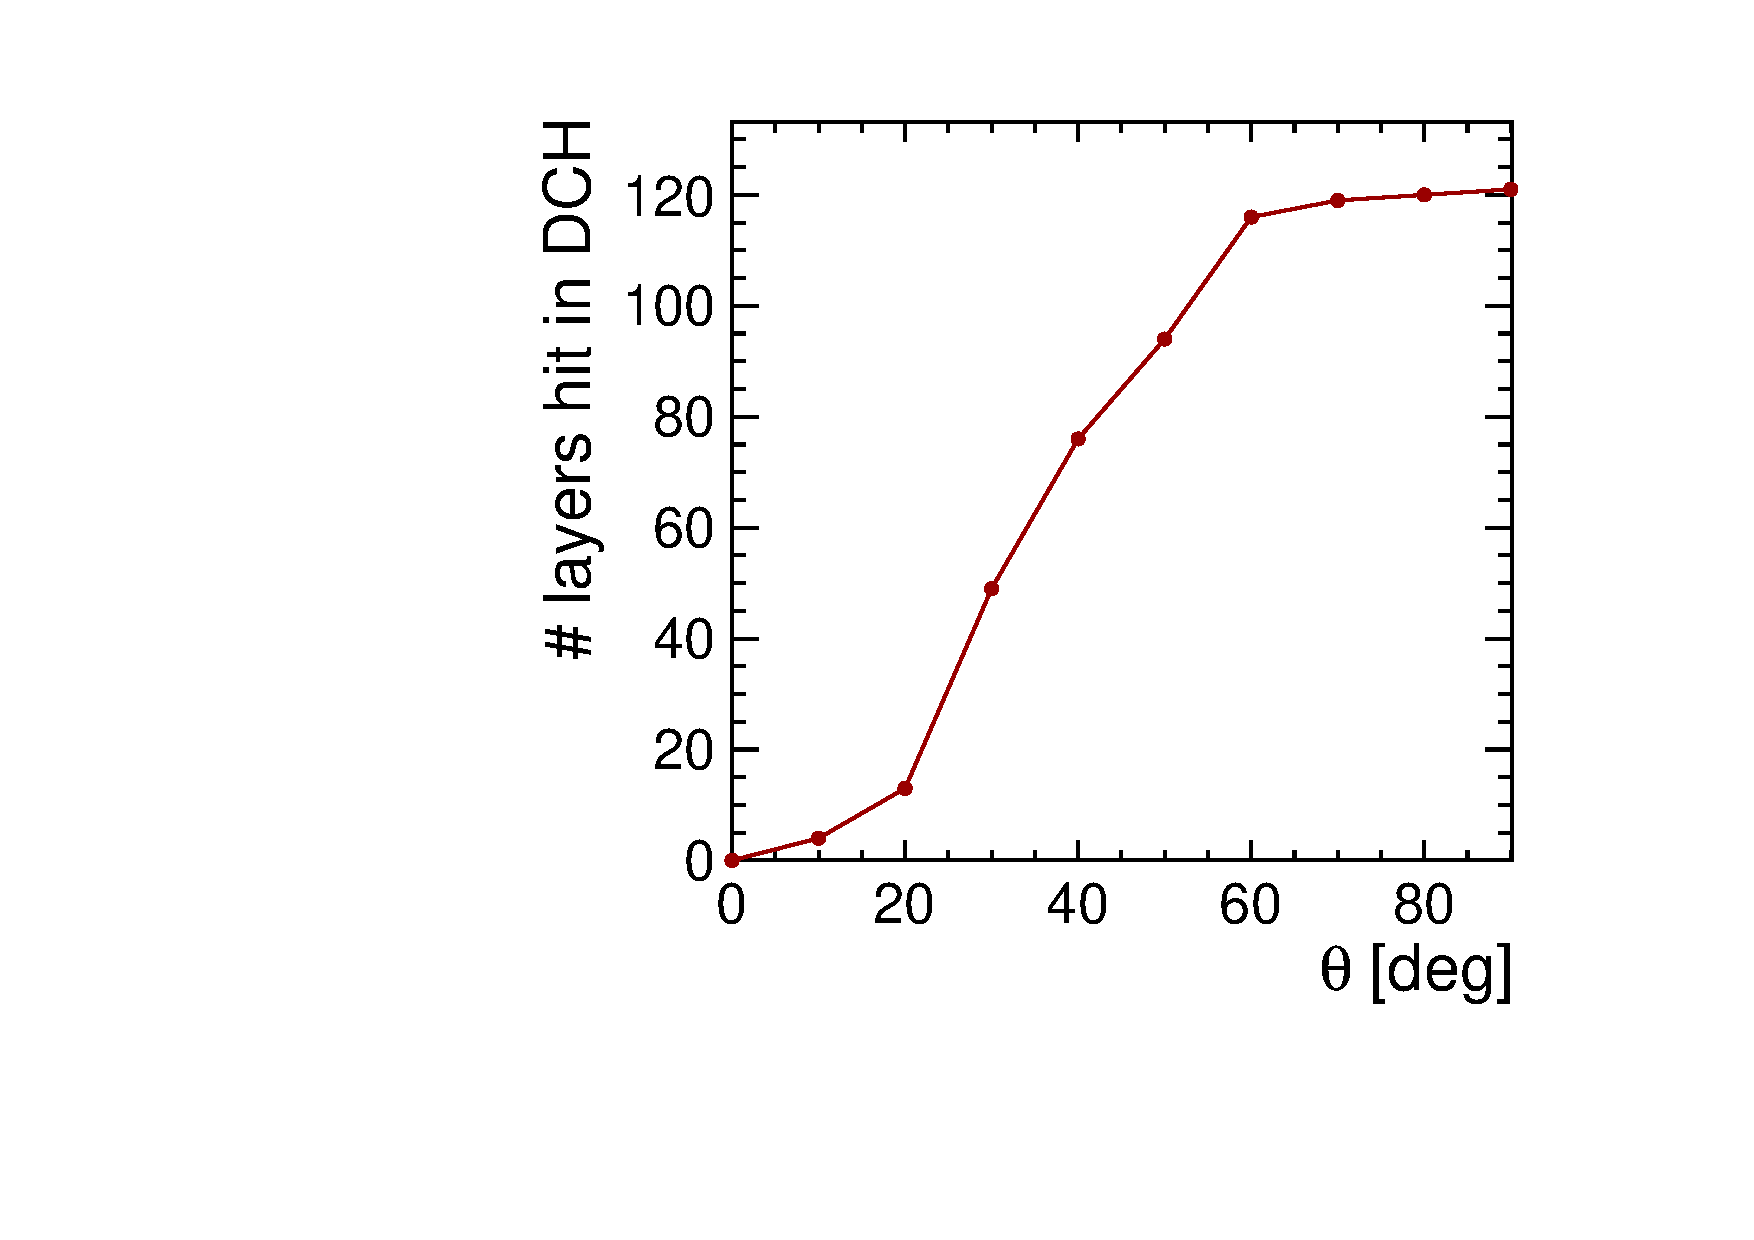
\includegraphics[width=\textwidth]{../figures/theta_nbHits_DCH.pdf} 	
		\end{block}
	\end{columns}
	
	
\end{frame}



%%%%%%%%%%%%%%%%%%%%%%%%%%%%%
%         SLIDE             %
%%%%%%%%%%%%%%%%%%%%%%%%%%%%%
\begin{frame}
	\frametitle{Background studies}

	\begin{itemize}
	\item The effect of incoherent $e+e-$ pairs on the interaction region (IR)
	\item Pairs generated using GuineaPig (c.f. Georgios Voutsinas)
	\item E\textsubscript{cm} = 365~GeV
	\item Total nb. of particles: $\sim6200$
	\end{itemize}		
	
	\begin{block}{Momentum distribution}
	\begin{columns}
	\column{0.5\textwidth}
		\centering
		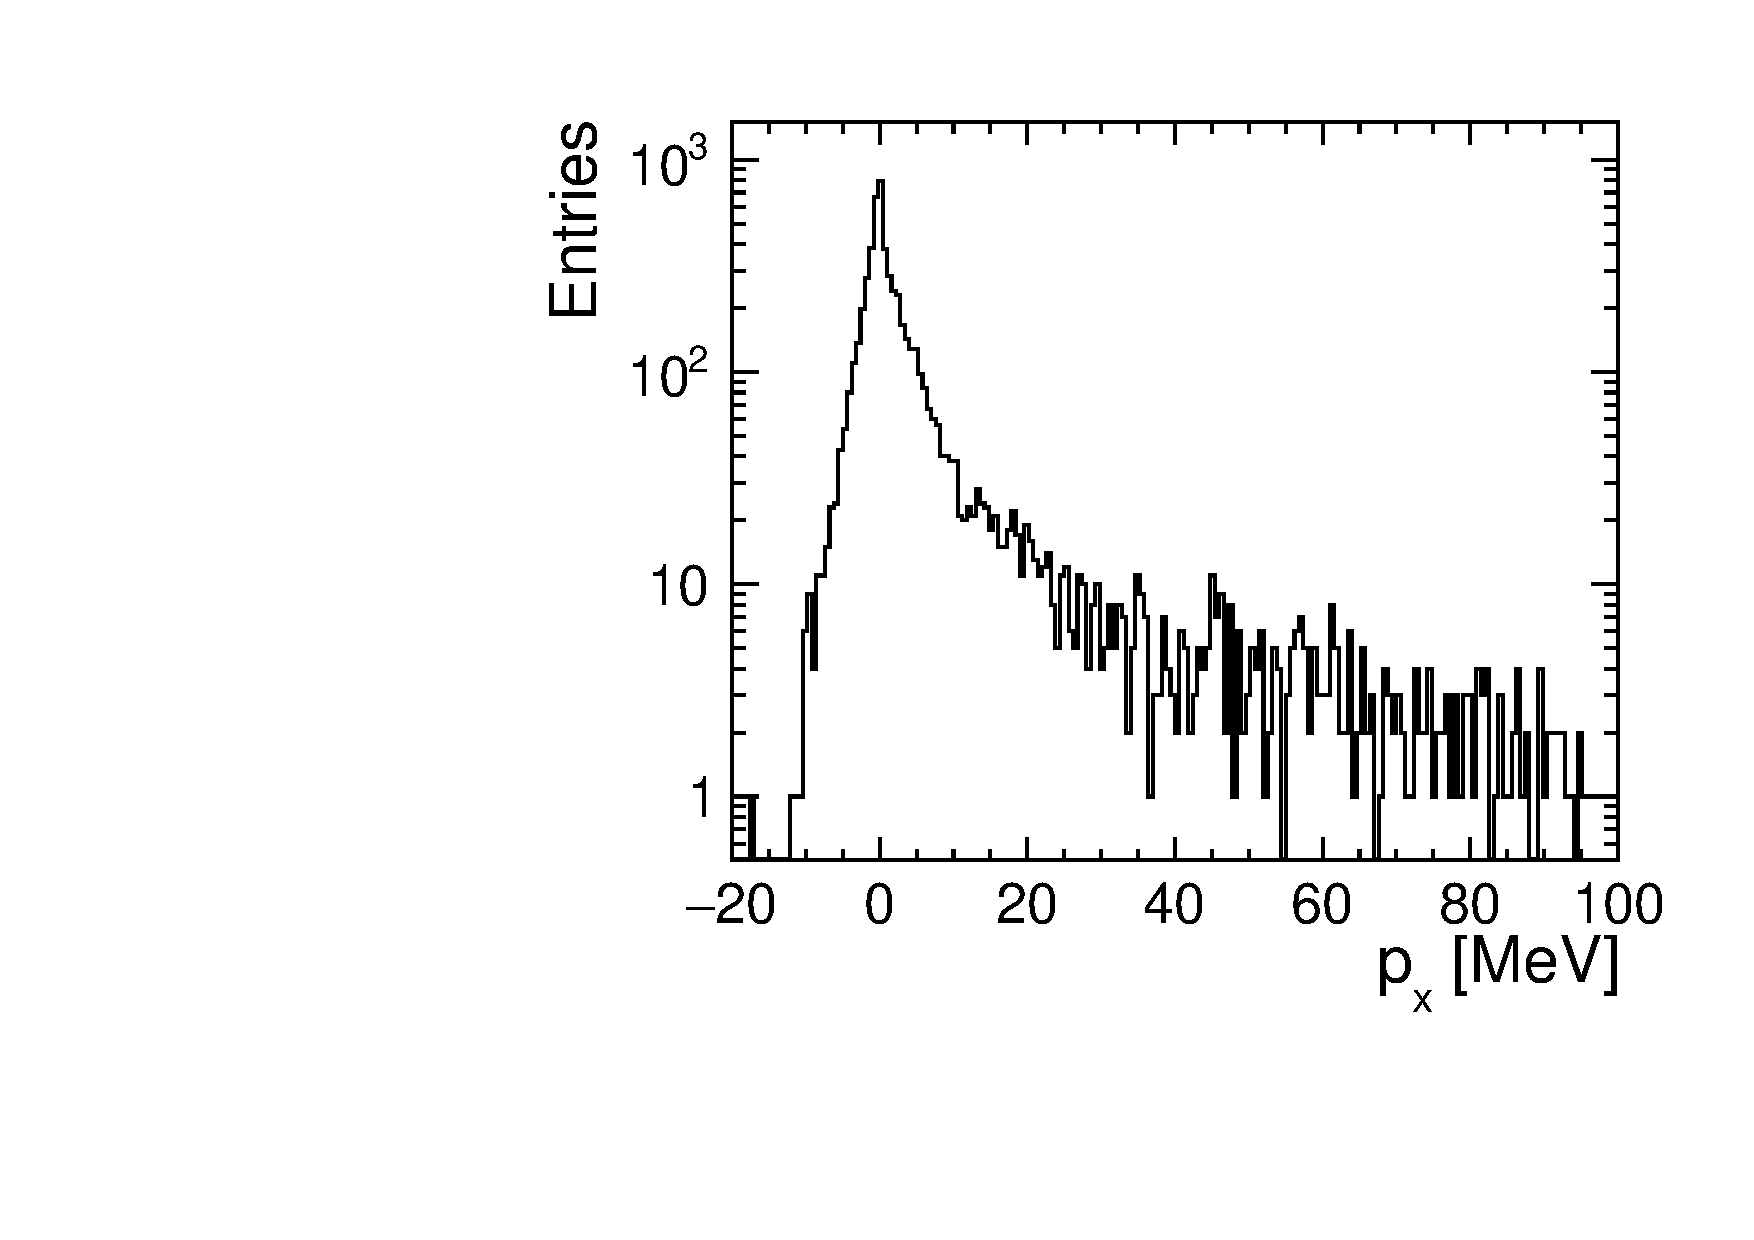
\includegraphics[width=0.7\textwidth]{../figures/incoherentPairs_px.pdf} \\									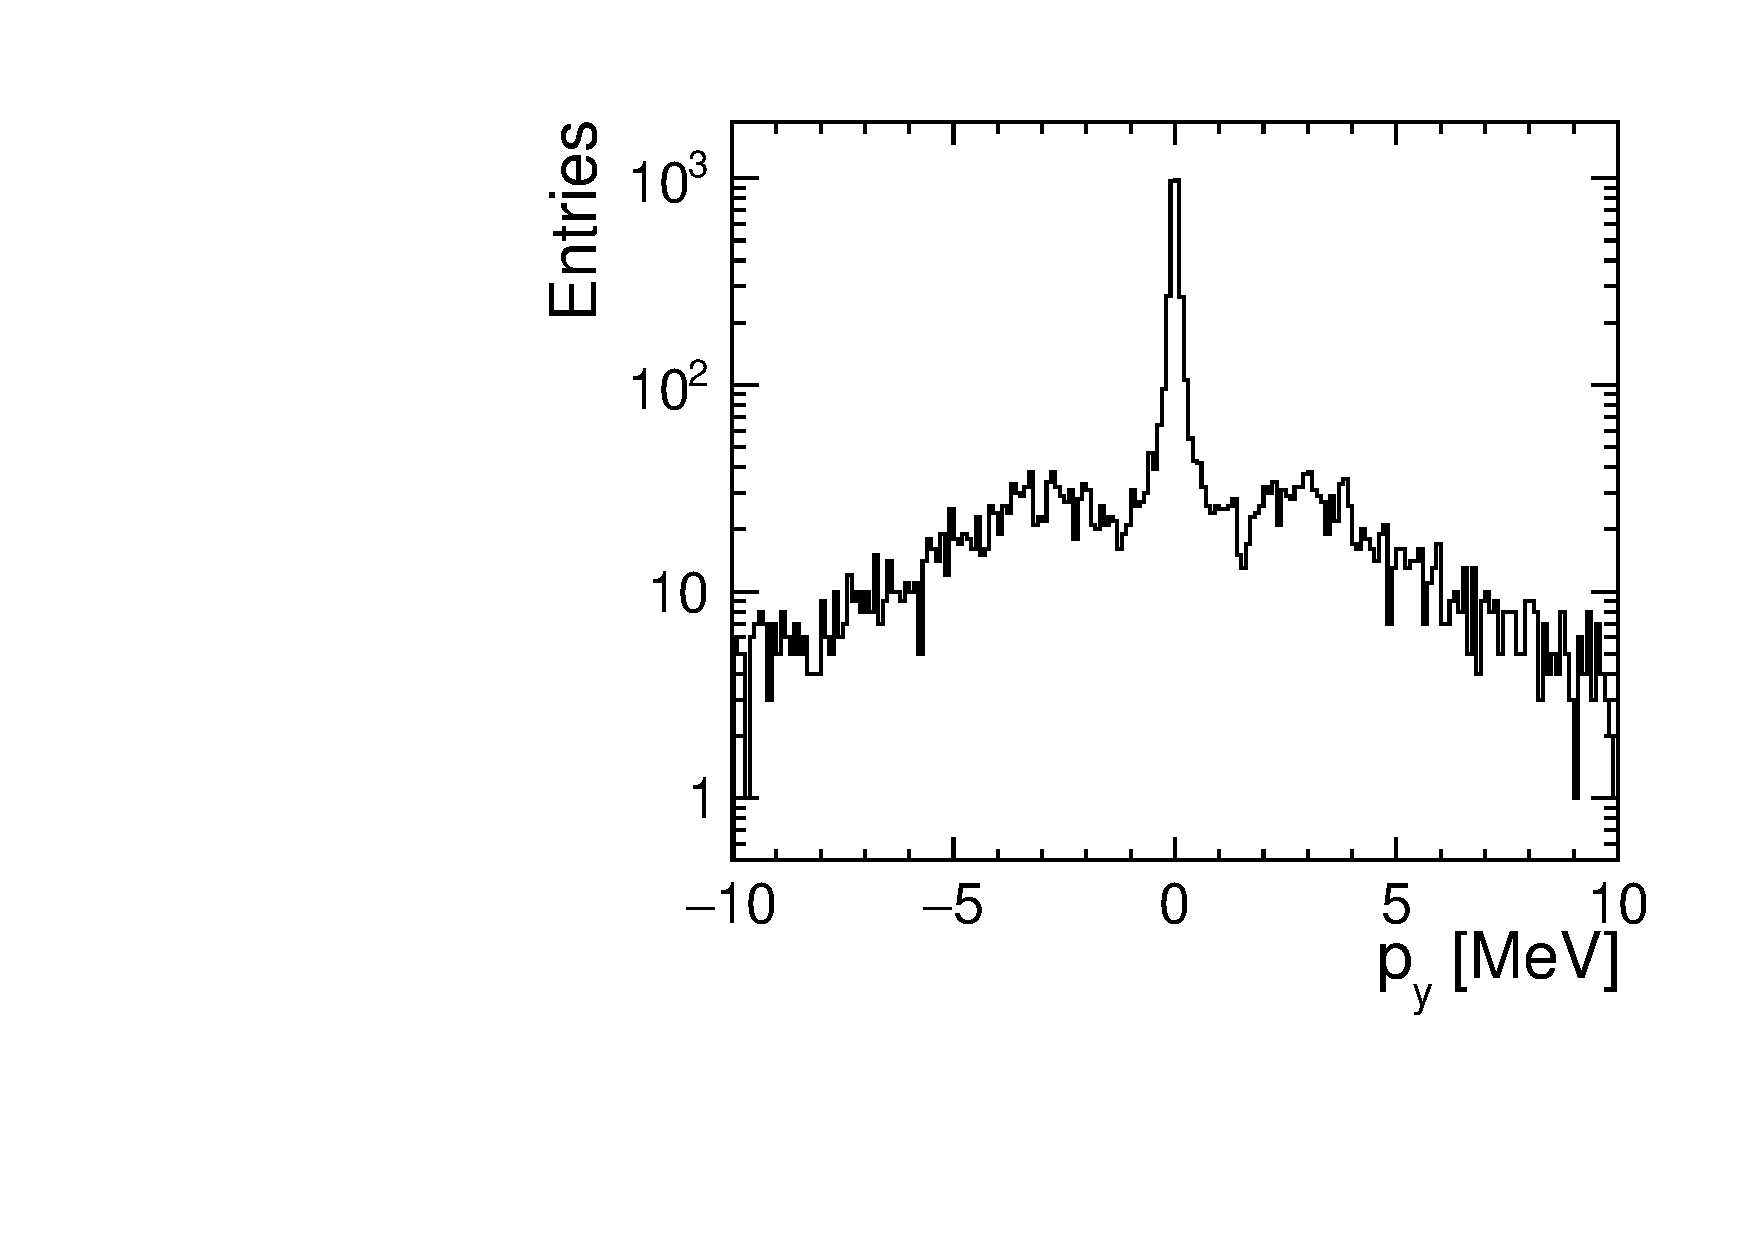
\includegraphics[width=0.7\textwidth]{../figures/incoherentPairs_py.pdf}
	\column{0.5\textwidth}
		\centering
		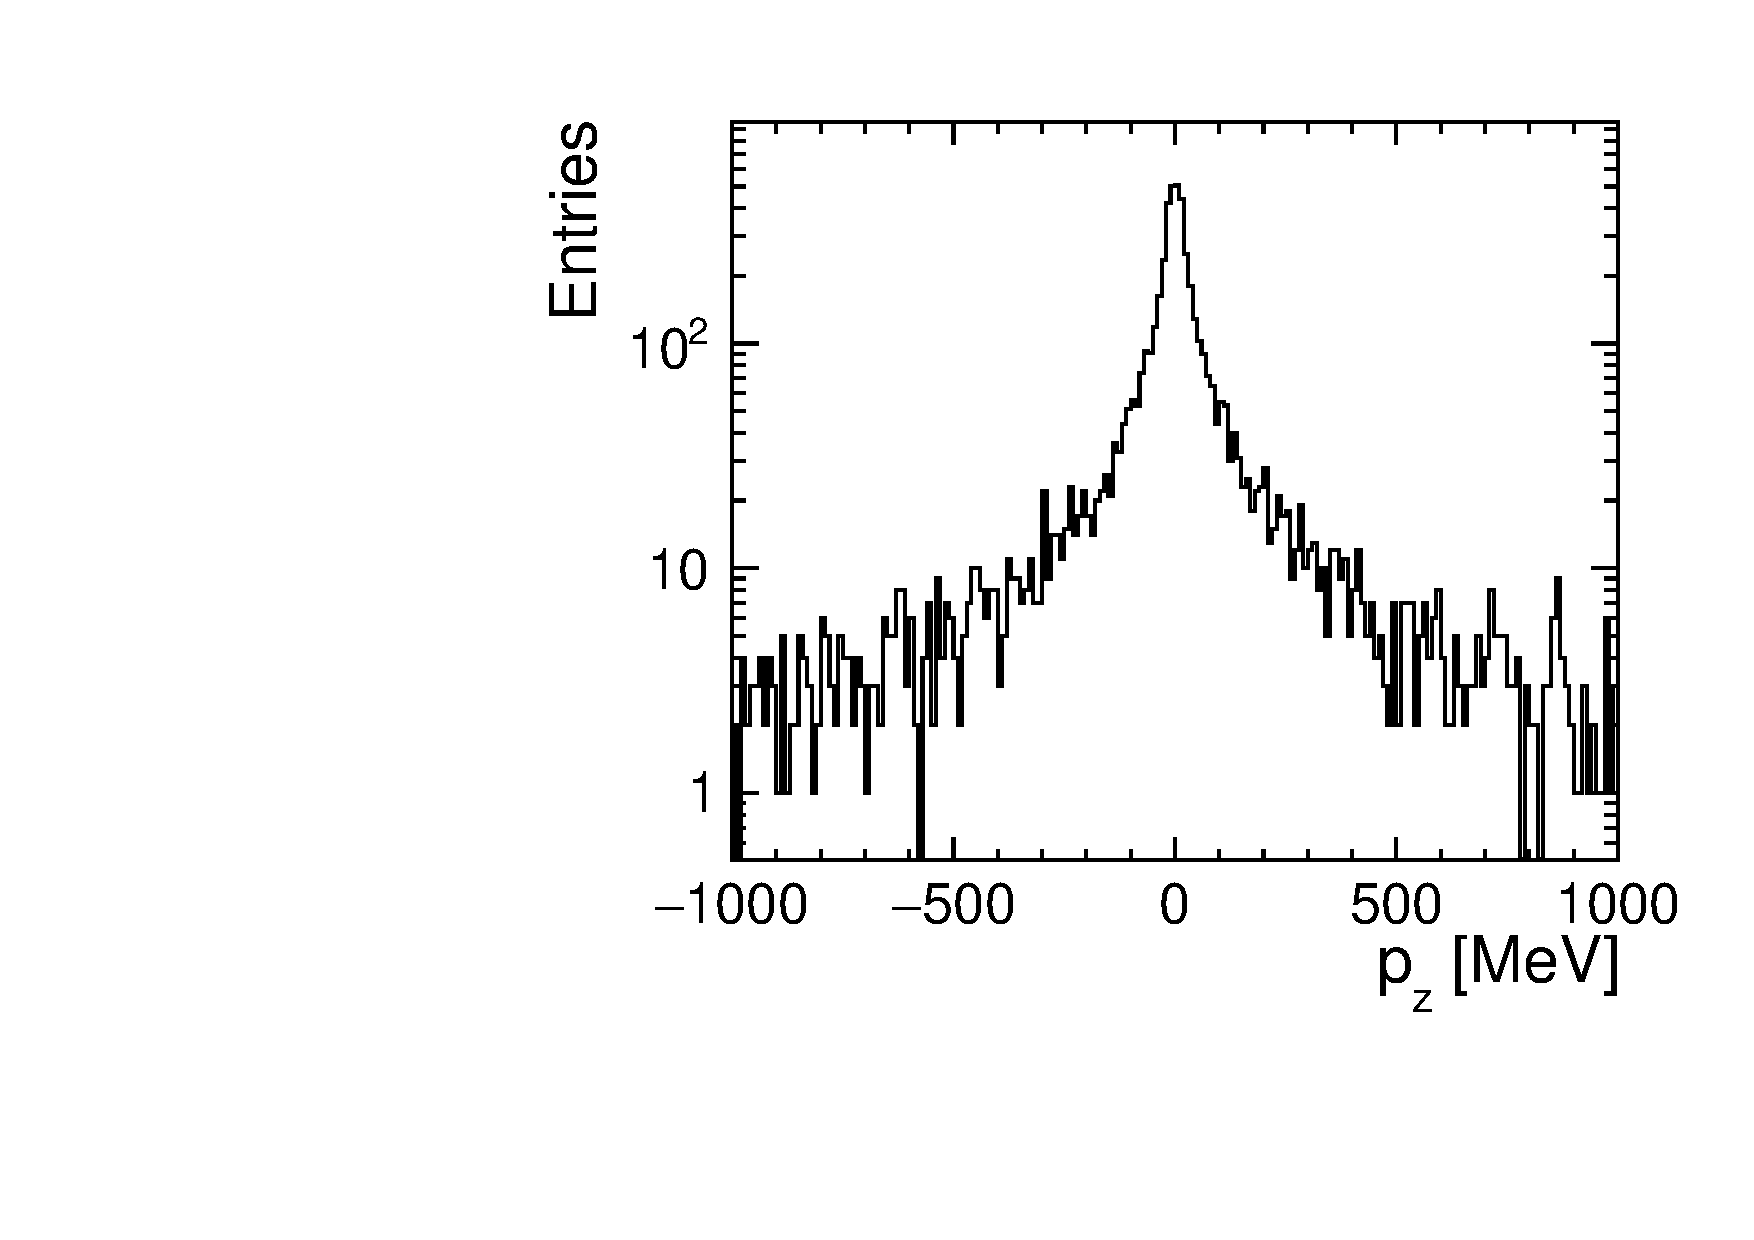
\includegraphics[width=0.7\textwidth]{../figures/incoherentPairs_pz.pdf}  \\
		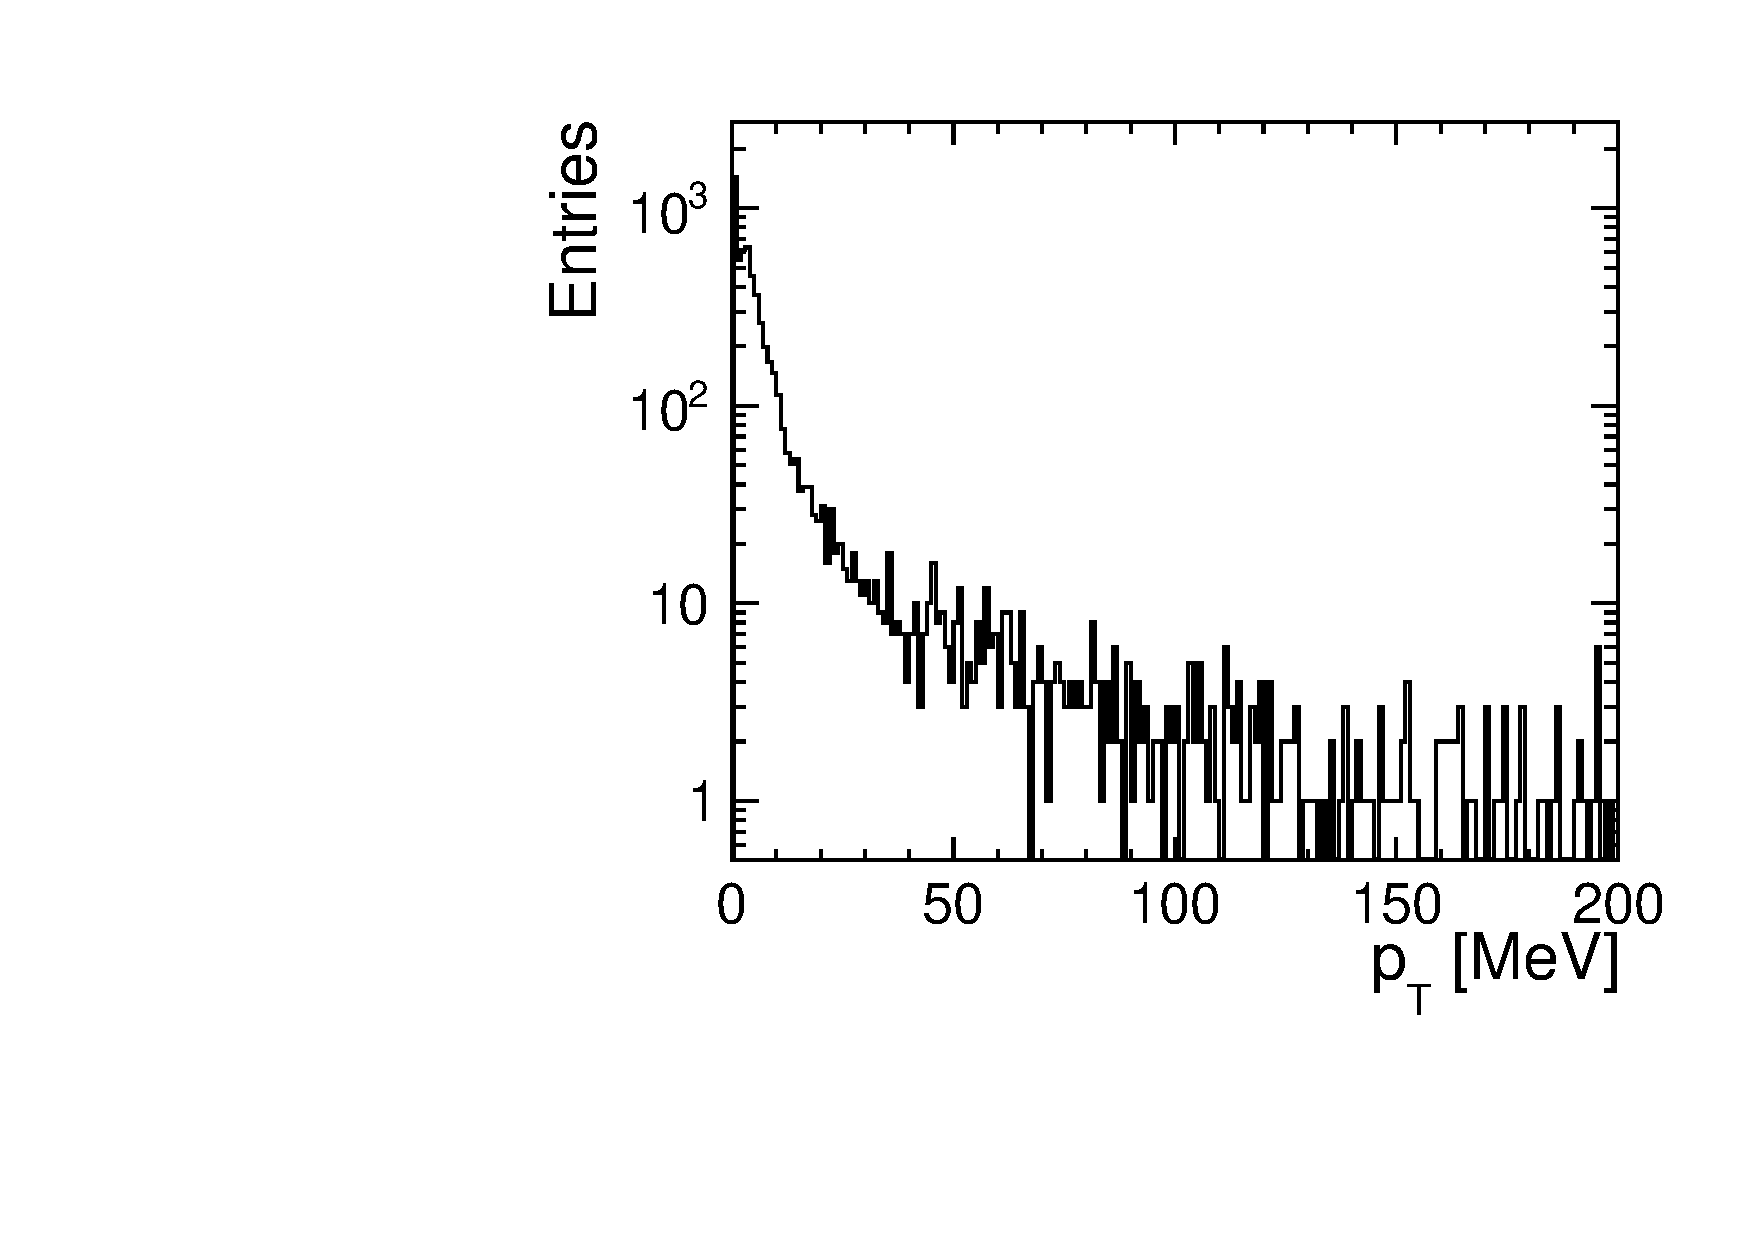
\includegraphics[width=0.7\textwidth]{../figures/incoherentPairs_pT.pdf} 

		\end{columns}	
	\end{block}
	
%	\begin{table}
%    \begin{adjustbox}{max width=\textwidth}
%      \begin{tabular}{l c}
%        \toprule
%        Events & Average number per BX \\
%        \hline
%        Total particles & 6160 \\
%        Hits in the VXD barrel & 2737 \\
%        Hits in the VXD endcap & 2537 \\
%        Hits in the DCH & 3345.7 \\
%        \bottomrule
%      \end{tabular}
%    \end{adjustbox}
%  \end{table}
	
\end{frame}

%%%%%%%%%%%%%%%%%%%%%%%%%%%%%
%         SLIDE             %
%%%%%%%%%%%%%%%%%%%%%%%%%%%%%
\begin{frame}
	\frametitle{Background studies for the VXD: work in progress}

	
	\begin{columns}
	\column{0.5\textwidth}
		\begin{itemize}
		\item Vertex Barrel
		\end{itemize}
		\centering
		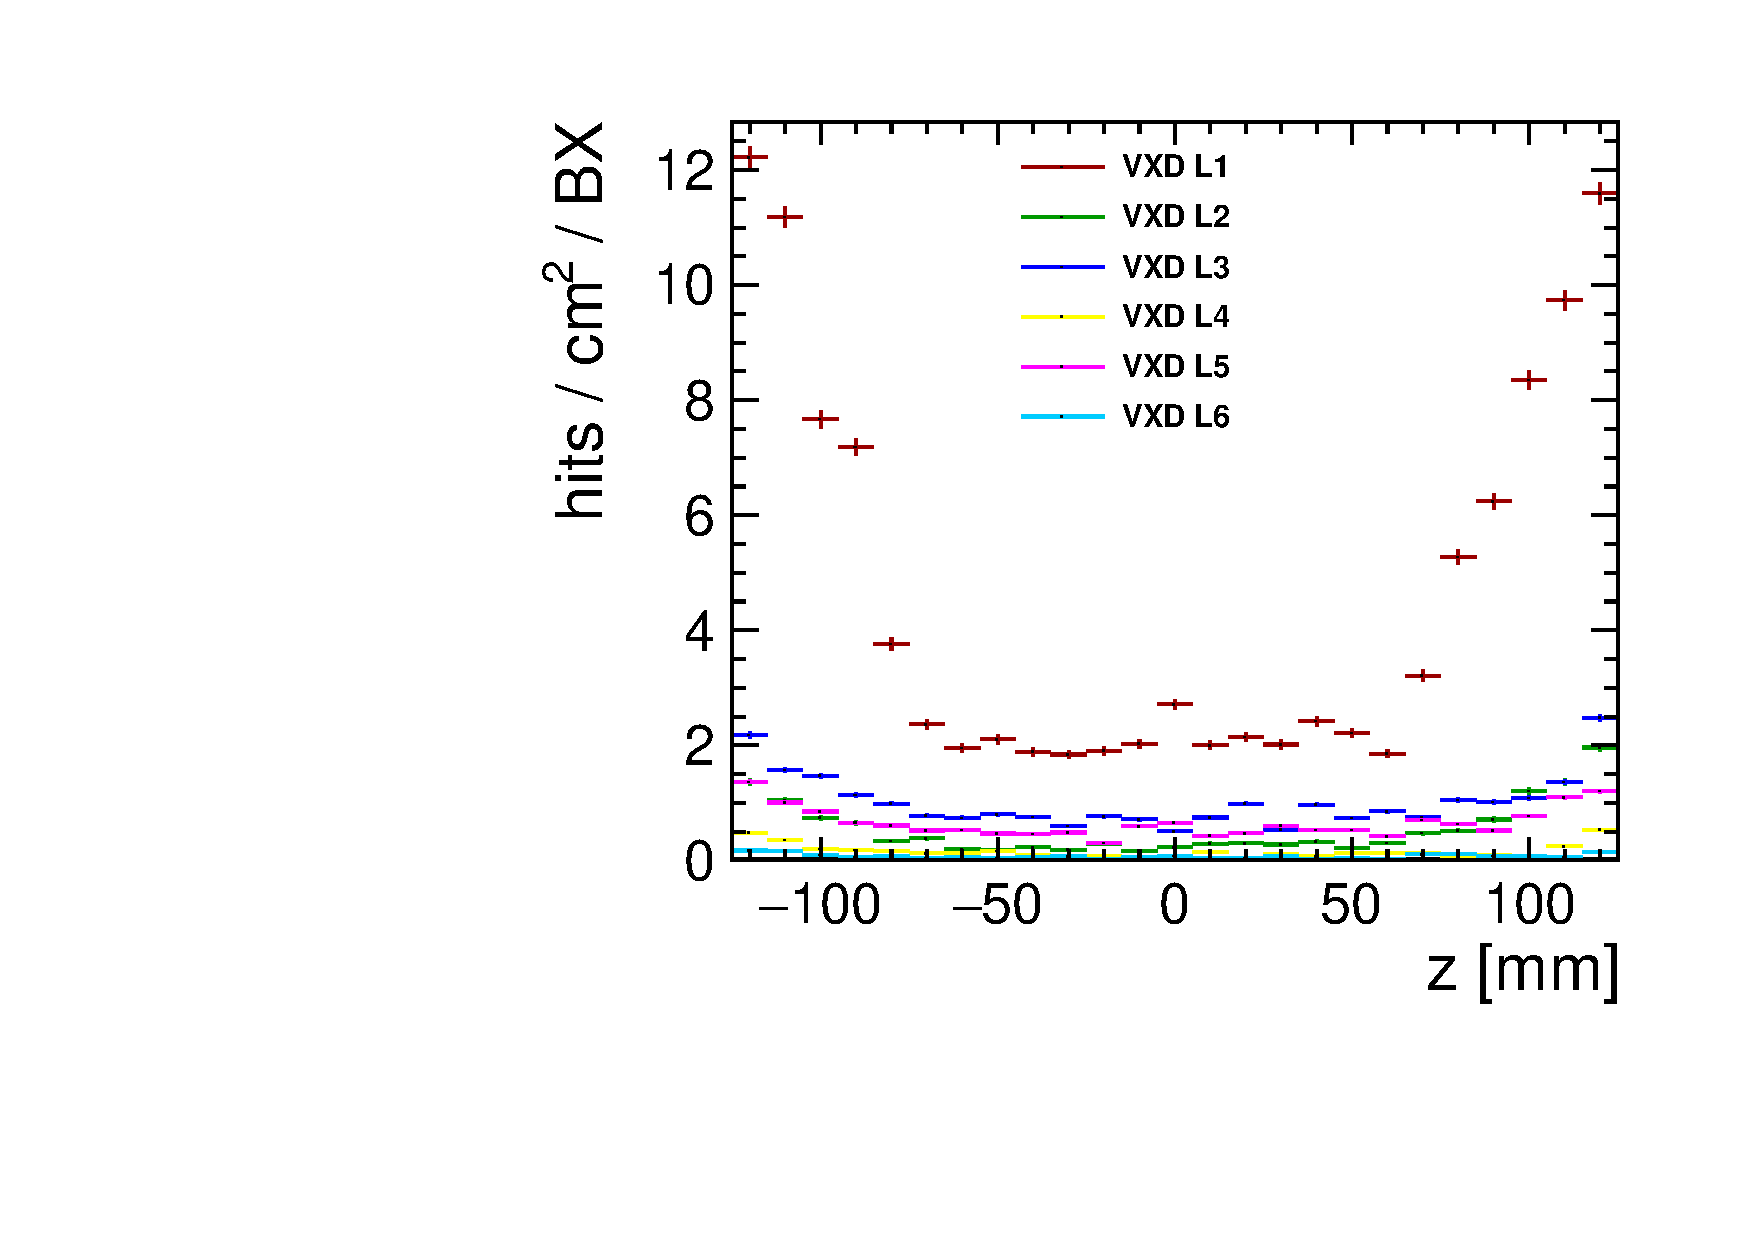
\includegraphics[width=\textwidth]{../figures/occupancy_VXD_barrel.pdf}
		
	\column{0.5\textwidth}
		\begin{itemize}
		\item Vertex Endcap
		\end{itemize}
		\centering
		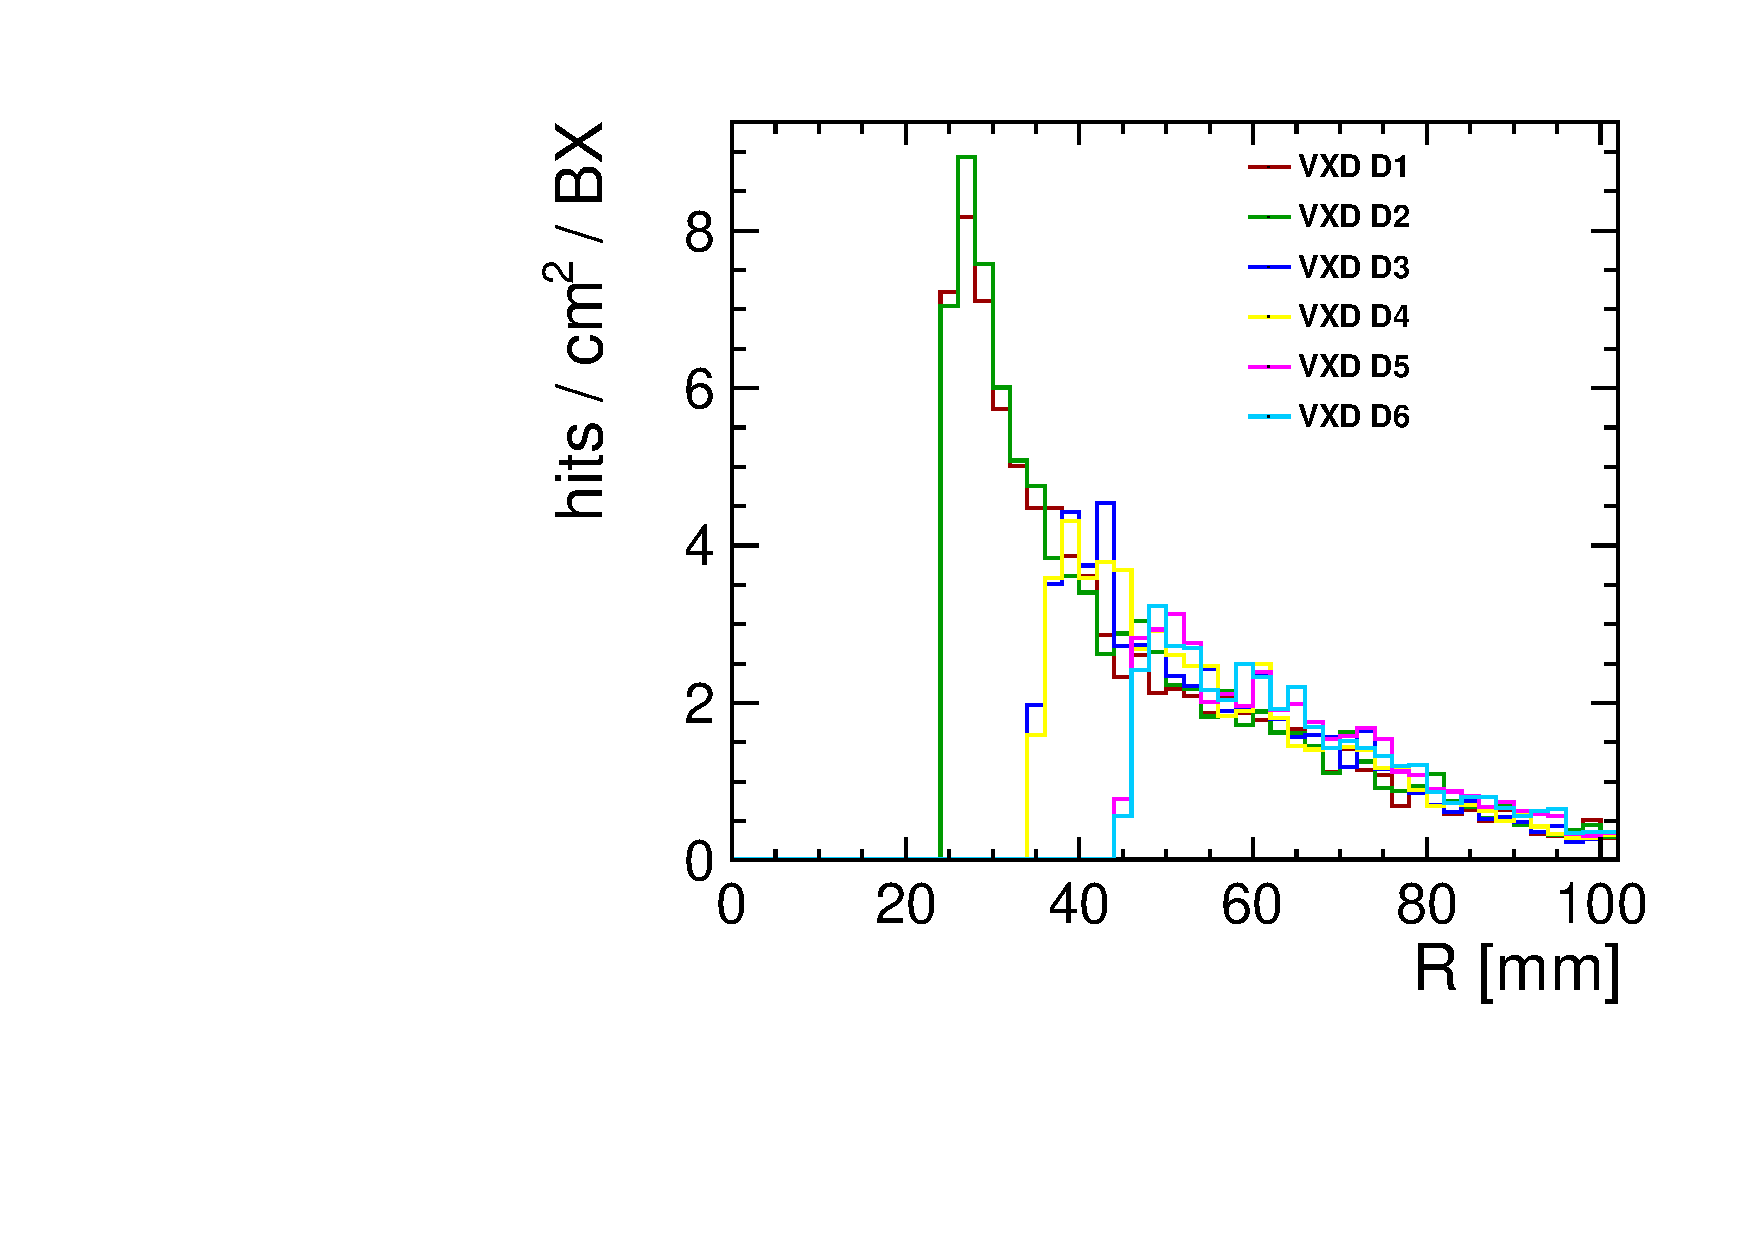
\includegraphics[width=\textwidth]{../figures/occupancy_VXD_endcap.pdf}
	\end{columns}
	
%	\begin{table}
%    \begin{adjustbox}{max width=\textwidth}
%      \begin{tabular}{l c}
%        \toprule
%        Detector & Total nb. of hits \\
%        \hline
%        Hits in the VXD barrel & 2737 \\
%        Hits in the VXD endcap & 2537 \\
%        \bottomrule
%      \end{tabular}
%    \end{adjustbox}
%  \end{table}
	
	
	\begin{itemize}
	\item Validations with ILCSoft in progress and promising
	\end{itemize}	
	
\end{frame}

%%%%%%%%%%%%%%%%%%%%%%%%%%%%%
%         SLIDE             %
%%%%%%%%%%%%%%%%%%%%%%%%%%%%%
\begin{frame}
	\frametitle{Background studies for the DCH: work in progress}

	\begin{columns}[t]
		\column{0.5\textwidth}
		\begin{itemize}
		\item Number of wires with different IDs recorded a signal
			\begin{itemize}
			\item Average: 3345.7 wires
			\end{itemize}
		\end{itemize}
	
		\centering
		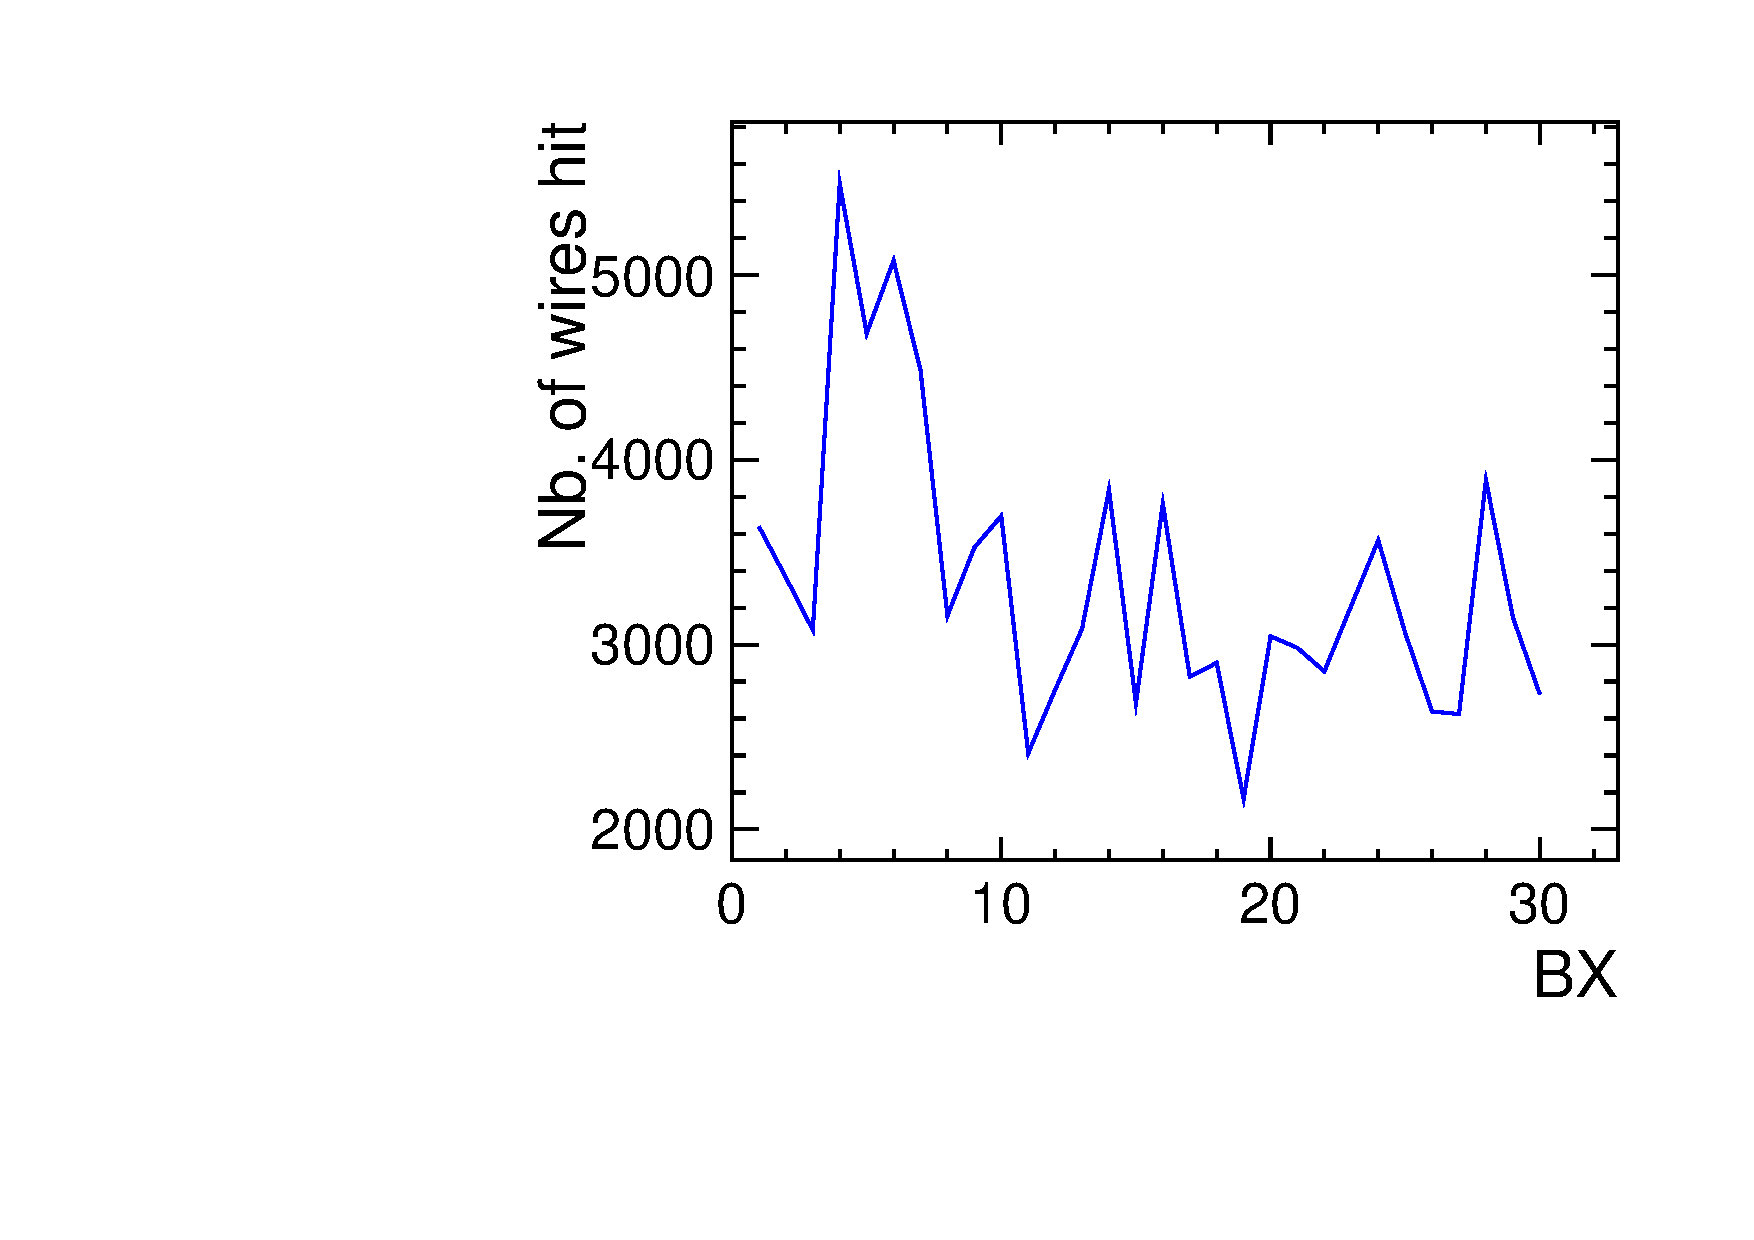
\includegraphics[width=\textwidth]{../figures/DCH/differentWires_hit_perBX.pdf}
	

		
		\column{0.5\textwidth}
		\begin{itemize}
		\item Number of hits recorded per wire in the first BX
		\item Mostly 1-hit per wire
		\item Several hits per wire: pile-up or same 
		\end{itemize}
		\centering
		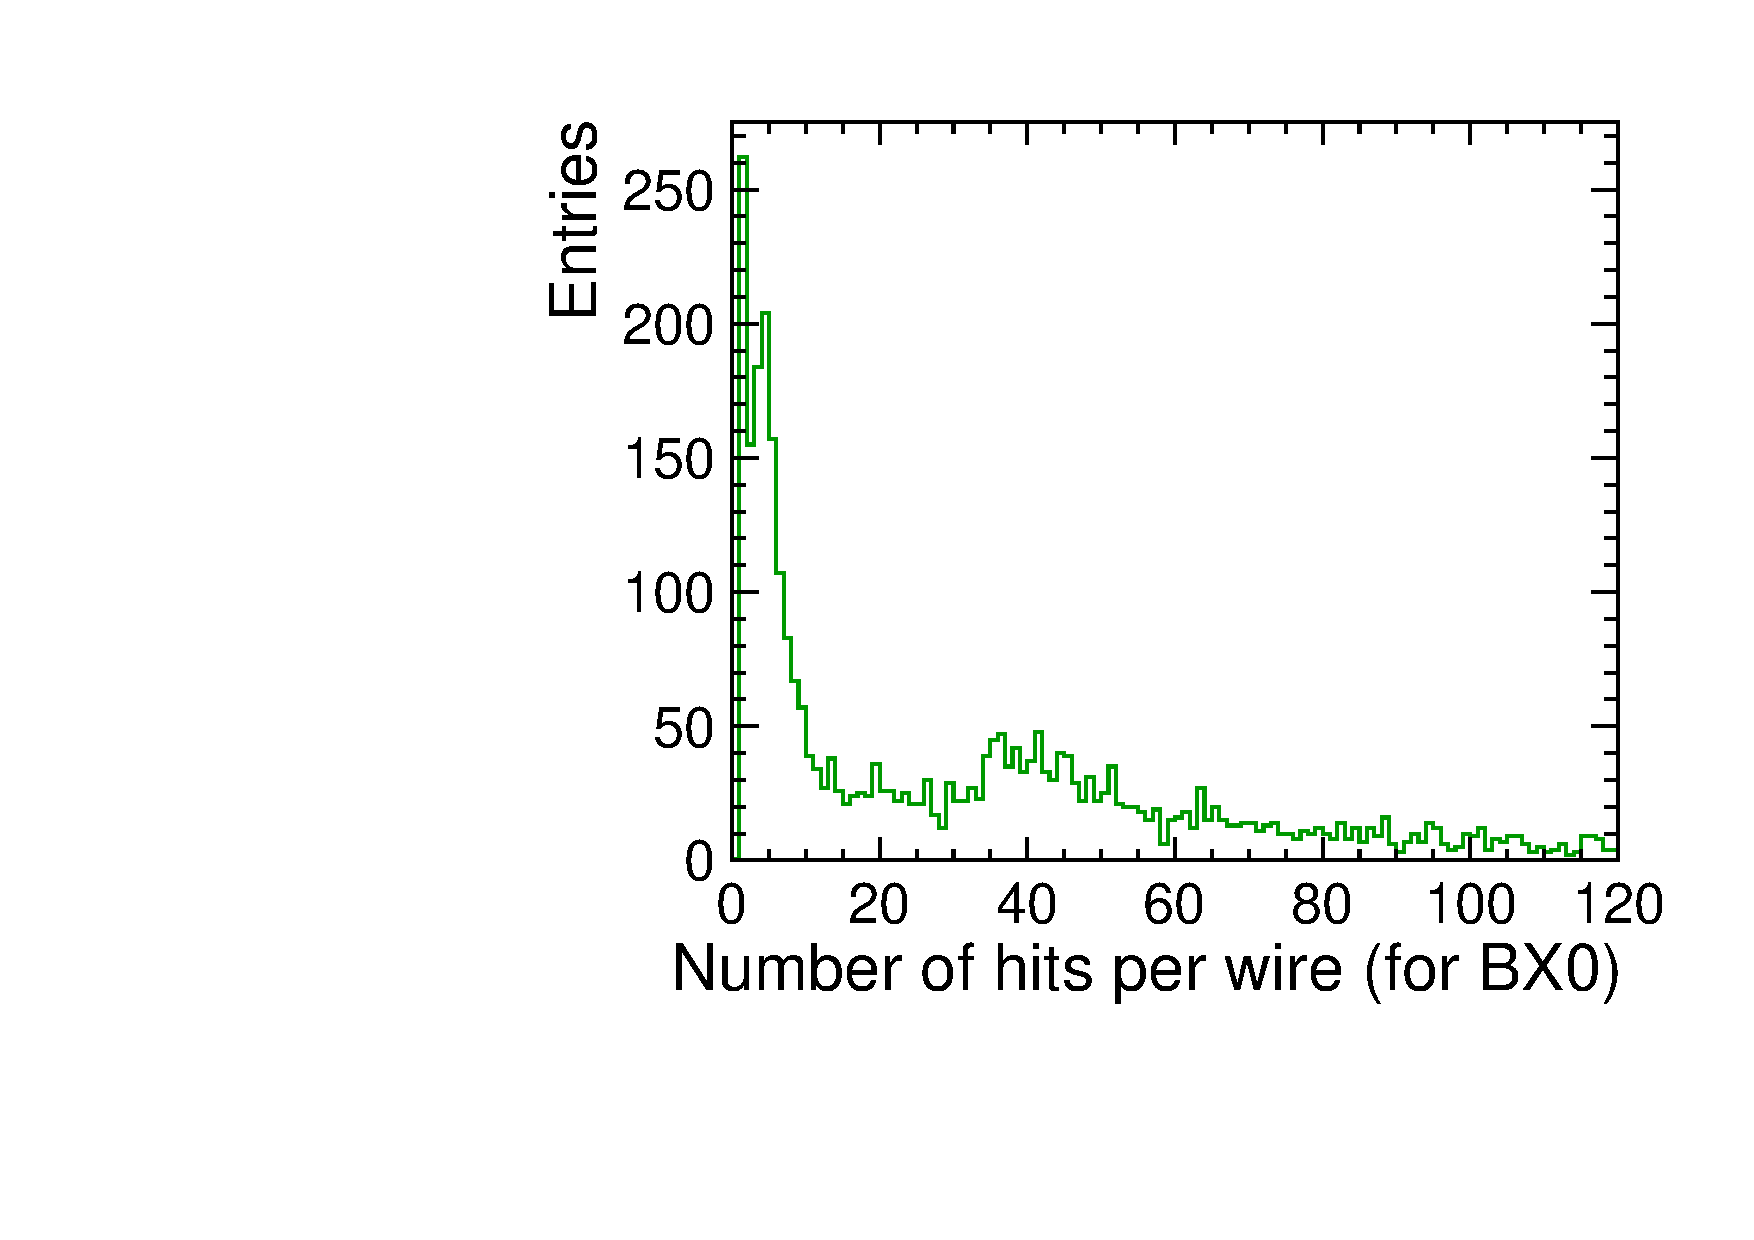
\includegraphics[width=\textwidth]{../figures/DCH/nb_hits_per_wire.pdf}
		
	\end{columns}
	
	\begin{itemize}
	\item To be investigated further: merging hits belonging to the same wire and having a drift time smaller than the maximum drift time in a cell.
	\item Occupancy as a function of the cell/voxel
	\end{itemize}		
	
\end{frame}

%%%%%%%%%%%%%%%%%%%%%%%%%%%%%
%         SLIDE             %
%%%%%%%%%%%%%%%%%%%%%%%%%%%%%
\begin{frame}
	\frametitle{Background studies for the DCH: number of hits per layer}

	
	\centering
	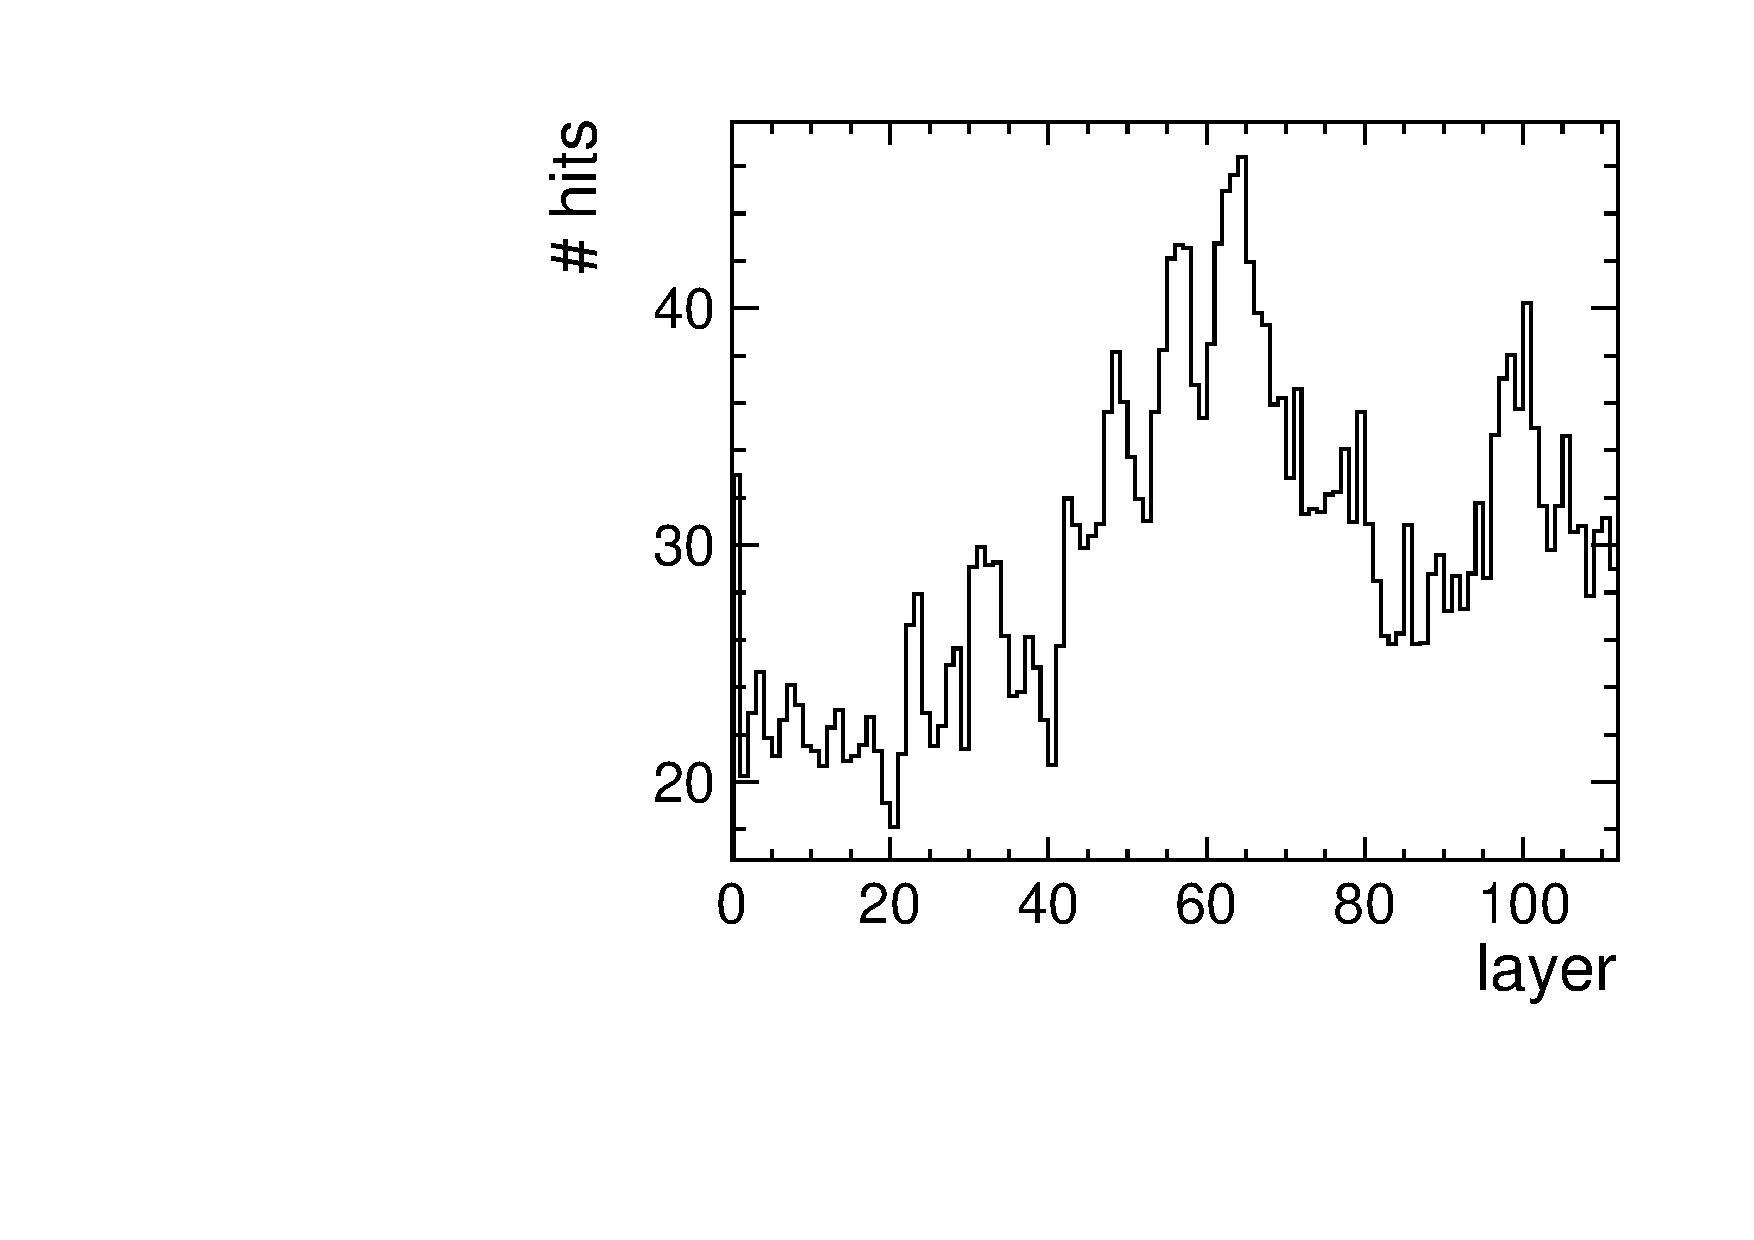
\includegraphics[width=\textwidth]{../figures/DCH/DCH_hits_layer.pdf}
		
	
	
\end{frame}

%%%%%%%%%%%%%%%%%%%%%%%%%%%%%
%         SLIDE             %
%%%%%%%%%%%%%%%%%%%%%%%%%%%%%
\label{lastslide}
\begin{frame}
  \frametitle{Summary \& Outlook}
  
	\begin{itemize}
	\item Full simulation of the FCCee-IDEA detector concept with FCCSW
	\item Implementation of the drift chamber 
		$\Rightarrow$ geometry, segmentation, simulation \& reconstuction
	\item Validations done and still ongoing 
	\item First physics studies:
		\begin{itemize}
		\item Impact of beam-induced backgrounds: e+e- incoherent pairs
	  	\item Estimation of the occupancy in the VXD and DCH with FCCSW and comparison with ILCSoft
	  	\end{itemize}
	\item Future work:
		\begin{itemize}
		\item Tracking
		\end{itemize}
  	\end{itemize}

\end{frame}


%%%%%%%%%%%%%%%%%%%%%%%%%%%%%%
%%         SLIDE             %
%%%%%%%%%%%%%%%%%%%%%%%%%%%%%%
%\begin{frame}
%  \frametitle{Number of times the same wire is hit per BX}
%
%  \begin{columns}
%  	\column{0.33\textwidth}	
%  	\begin{itemize}
%  	\item BX 0
%  	\end{itemize}
%	\centering
%	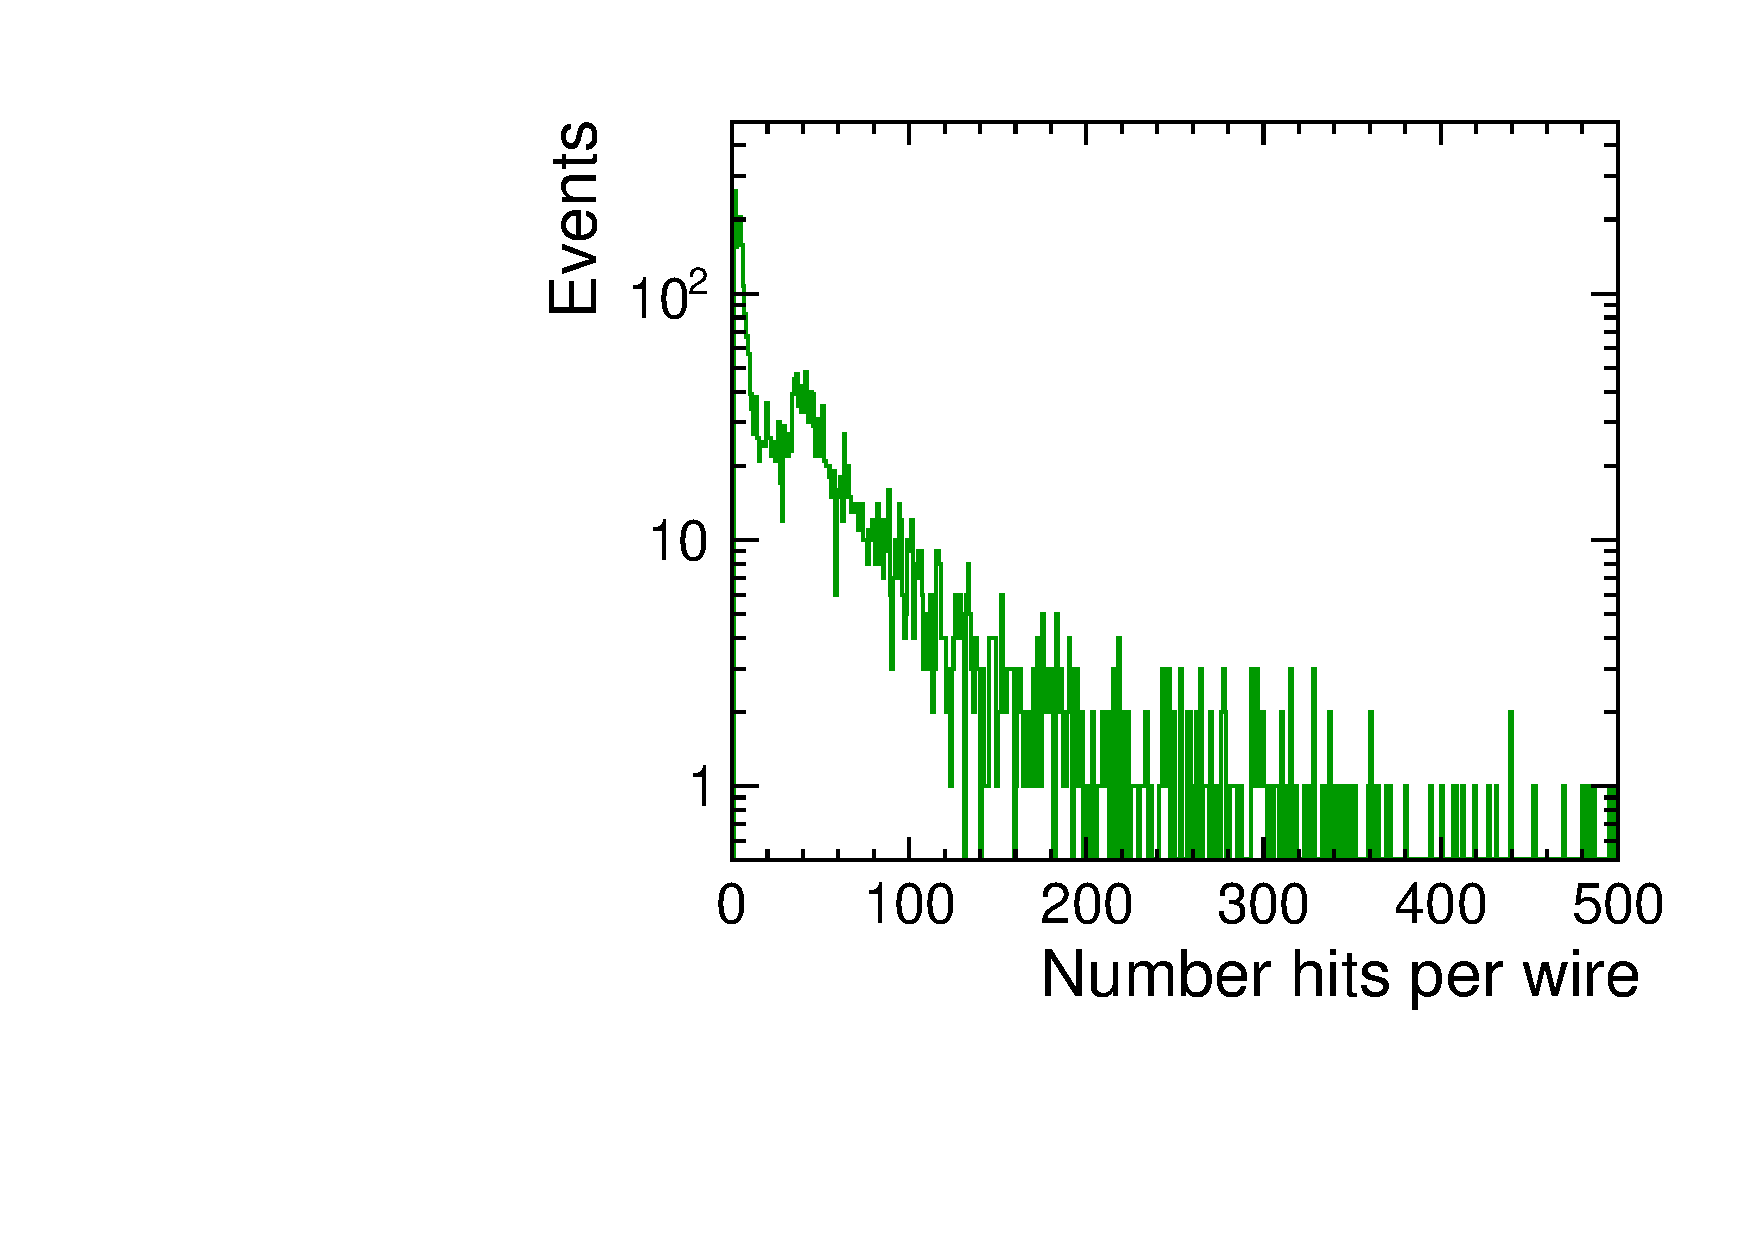
\includegraphics[width=\textwidth]{../figures/DCH/nbWires_BX0.pdf}
%	
%	\column{0.33\textwidth}
%	\begin{itemize}
%  	\item BX 1
%  	\end{itemize}
%	\centering
%	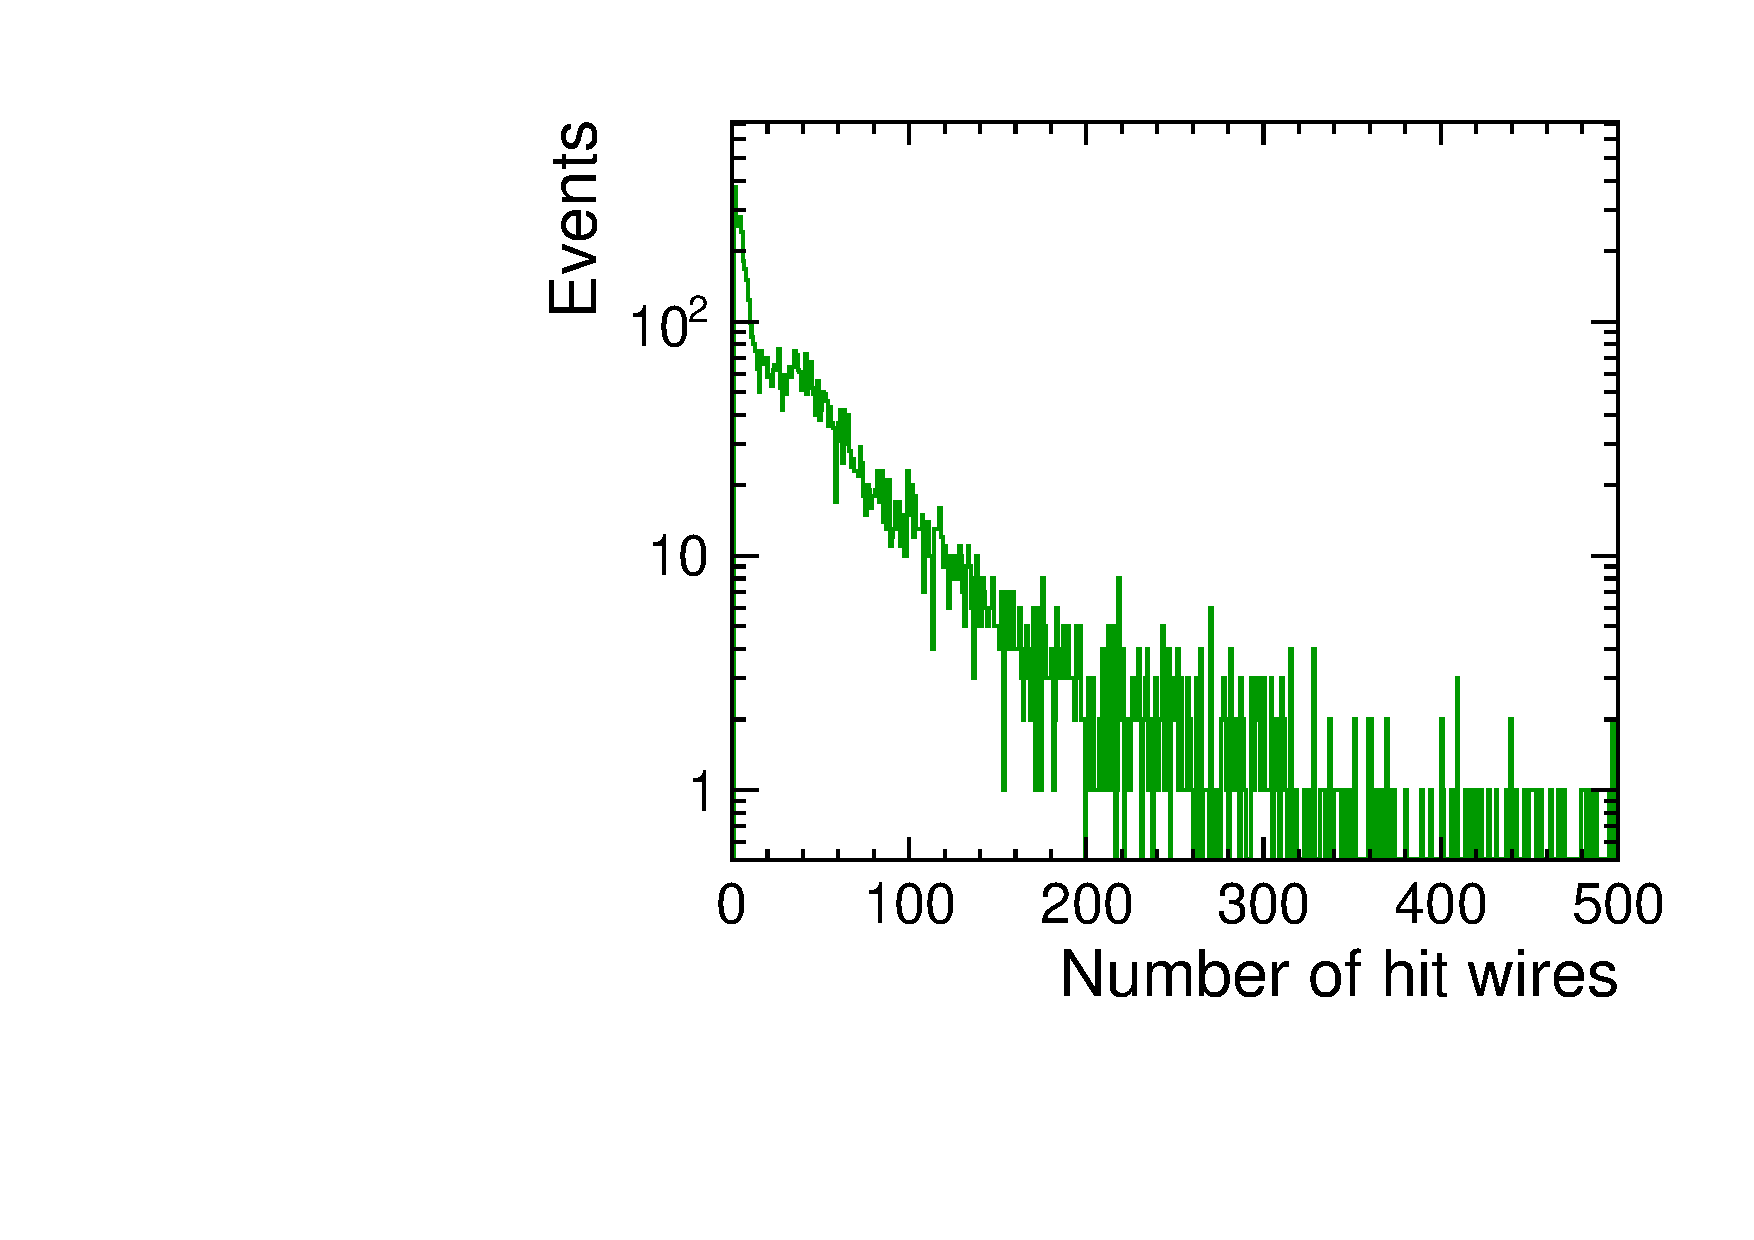
\includegraphics[width=\textwidth]{../figures/DCH/nbWires_BX1.pdf}
%	
%	\column{0.33\textwidth}	
%  	\begin{itemize}
%  	\item BX 2
%  	\end{itemize}
%	\centering
%	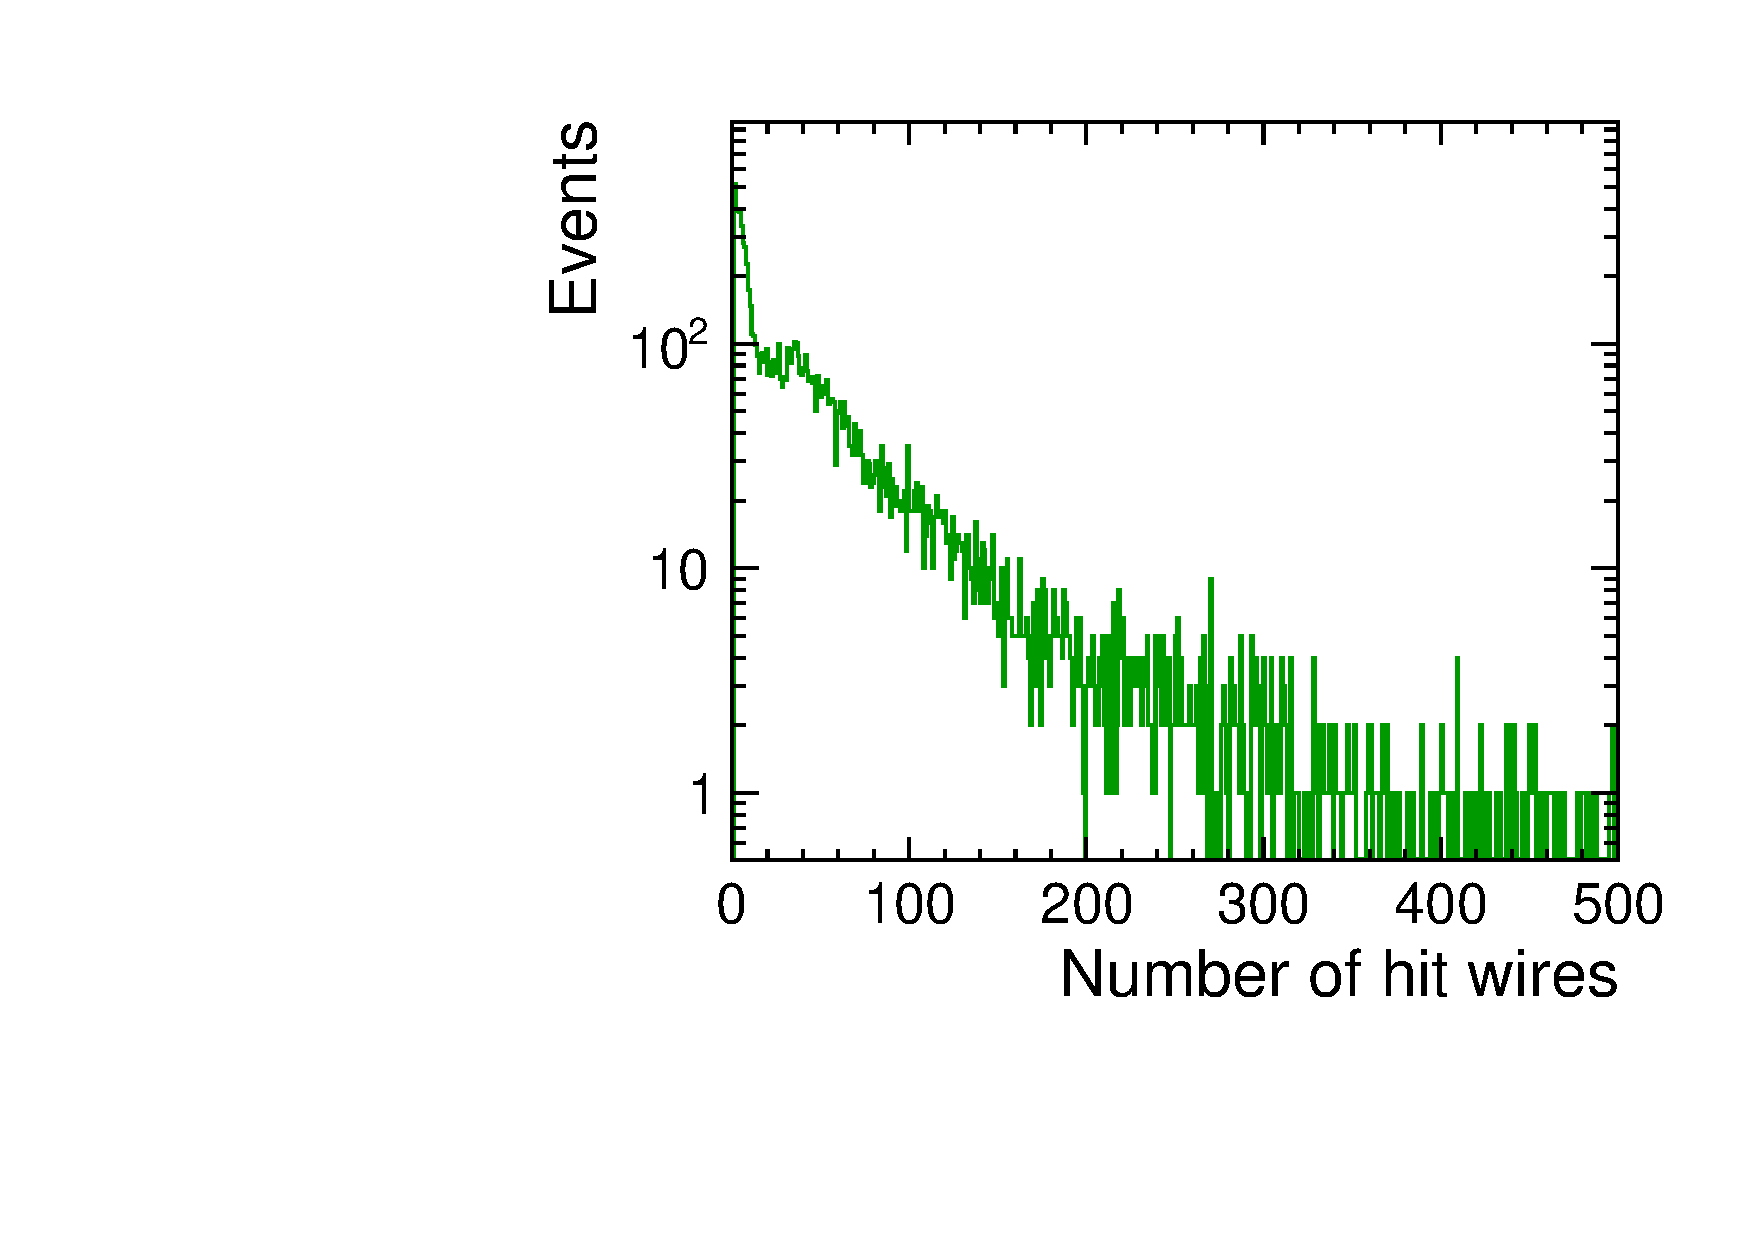
\includegraphics[width=\textwidth]{../figures/DCH/nbWires_BX2.pdf}
%  \end{columns}
%
%\end{frame}
%
%%%%%%%%%%%%%%%%%%%%%%%%%%%%%%
%%         SLIDE             %
%%%%%%%%%%%%%%%%%%%%%%%%%%%%%%
%\begin{frame}
%  \frametitle{Material Budget: Full Detector}
%
%  \begin{columns}
%  	\column{0.33\textwidth}	
%	\centering
%	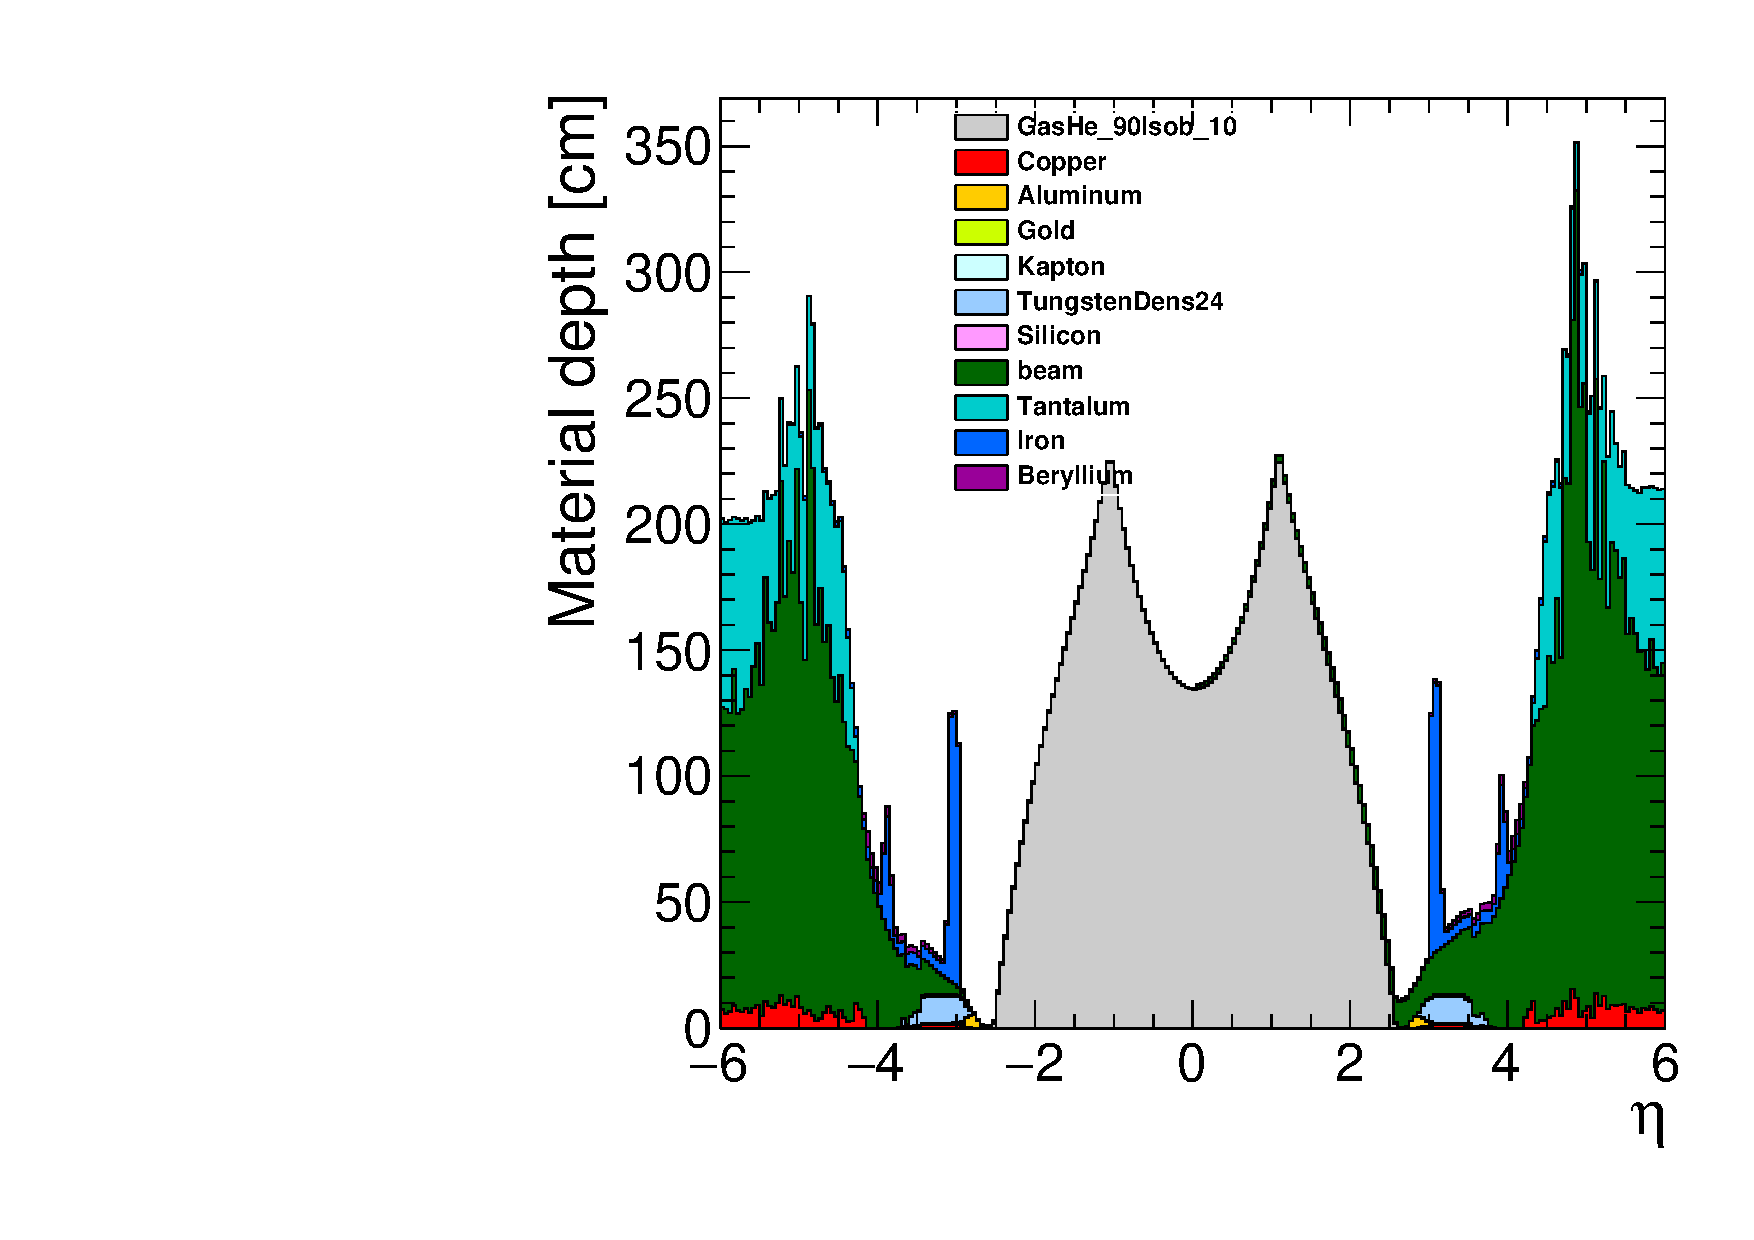
\includegraphics[width=\textwidth]{../figures/material/depth.pdf}\\
%	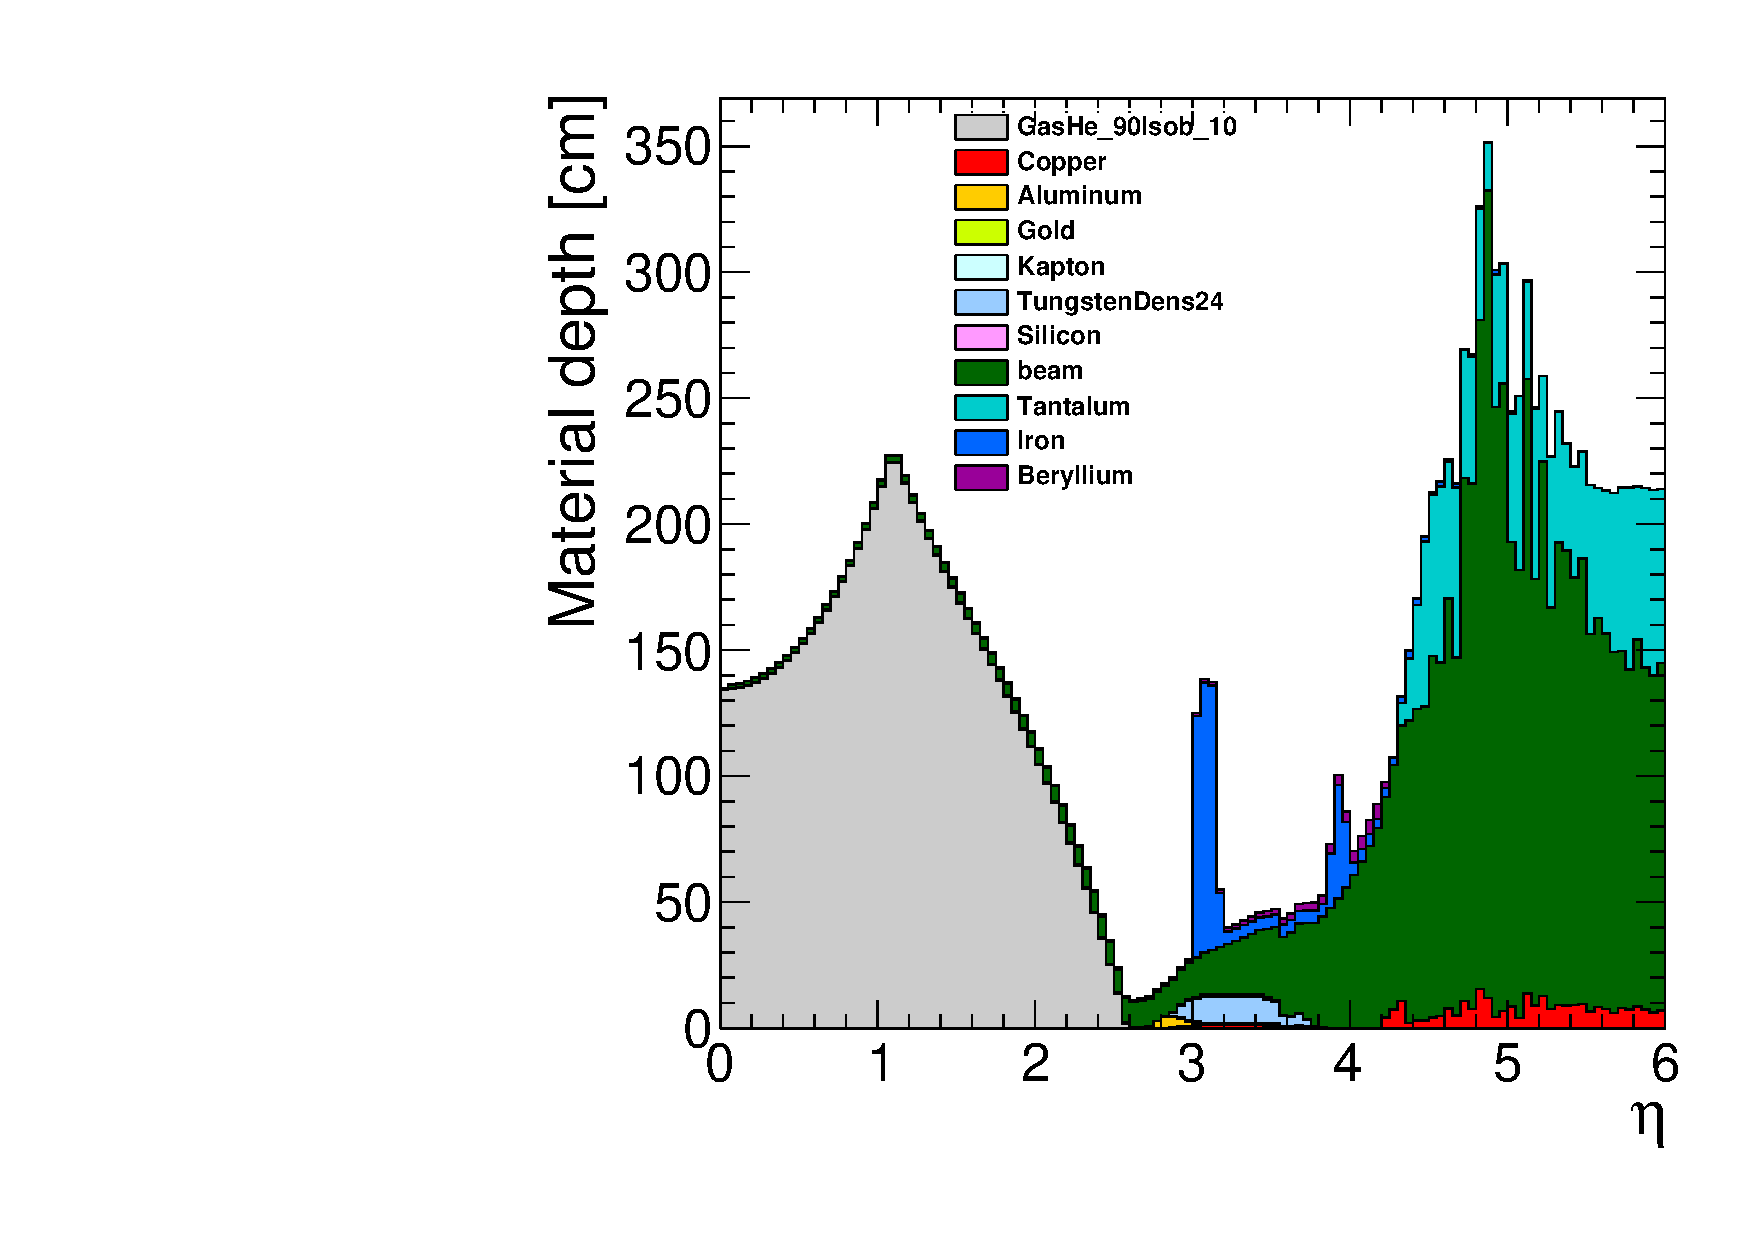
\includegraphics[width=\textwidth]{../figures/material/depthpos.pdf}
%	
%	\column{0.33\textwidth}	
%	\centering
%	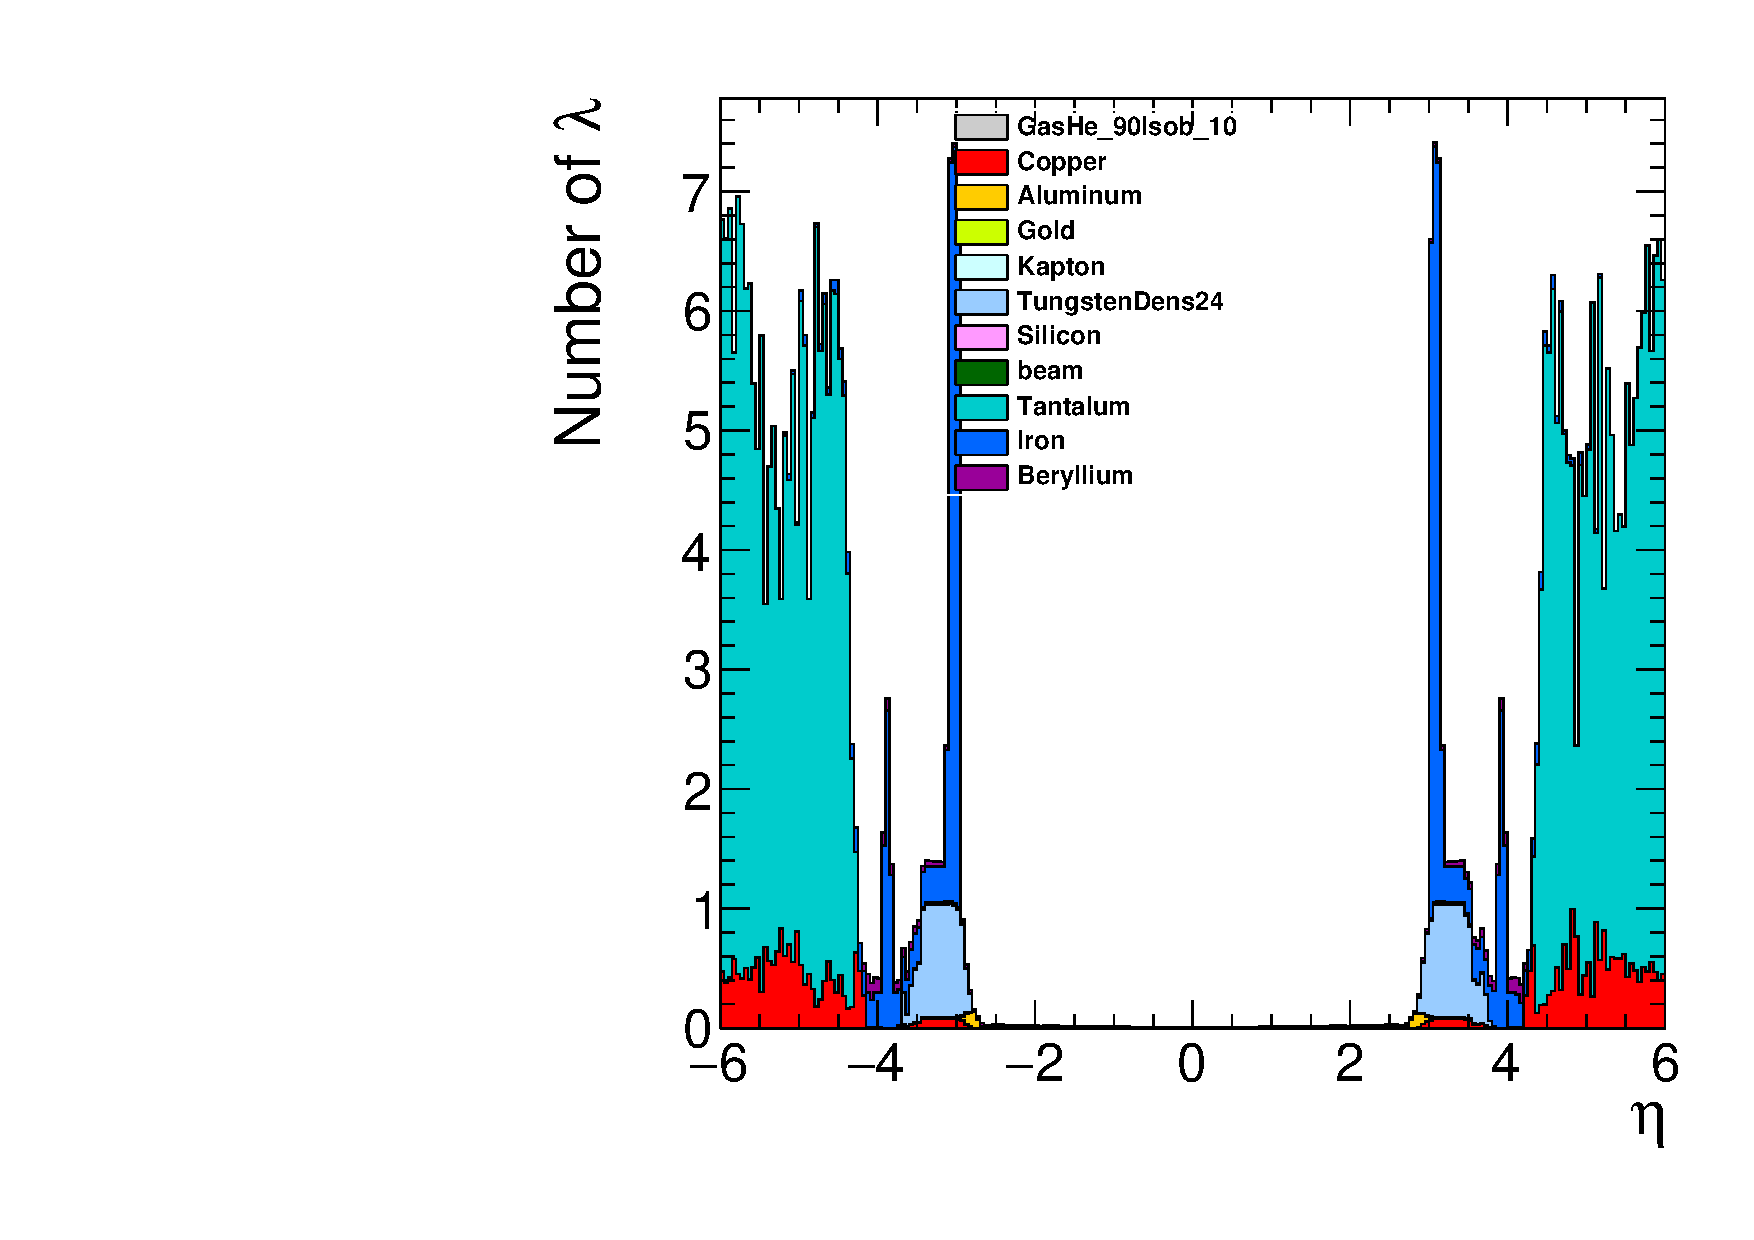
\includegraphics[width=\textwidth]{../figures/material/lambda.pdf}\\
%	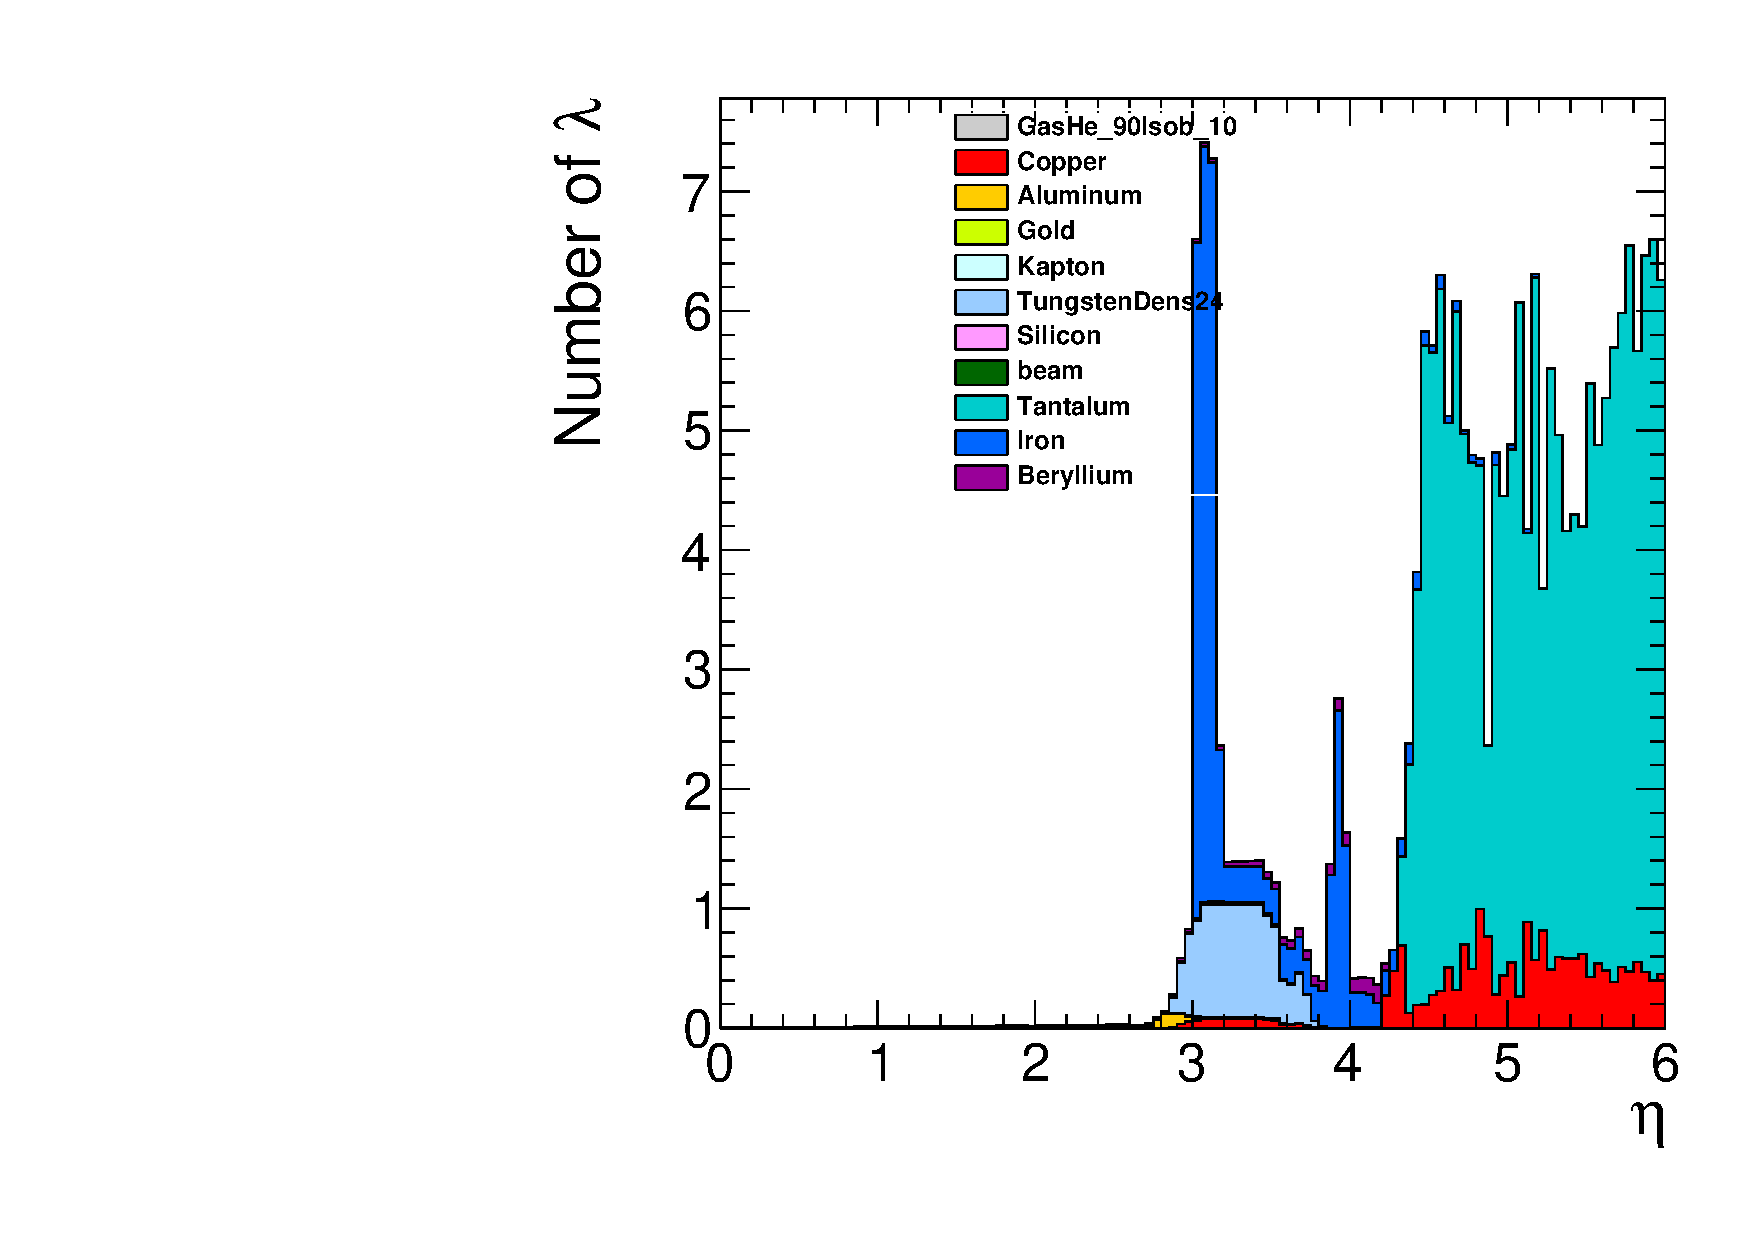
\includegraphics[width=\textwidth]{../figures/material/lambdapos.pdf}
%	
%	\column{0.33\textwidth}	
%	\centering
%	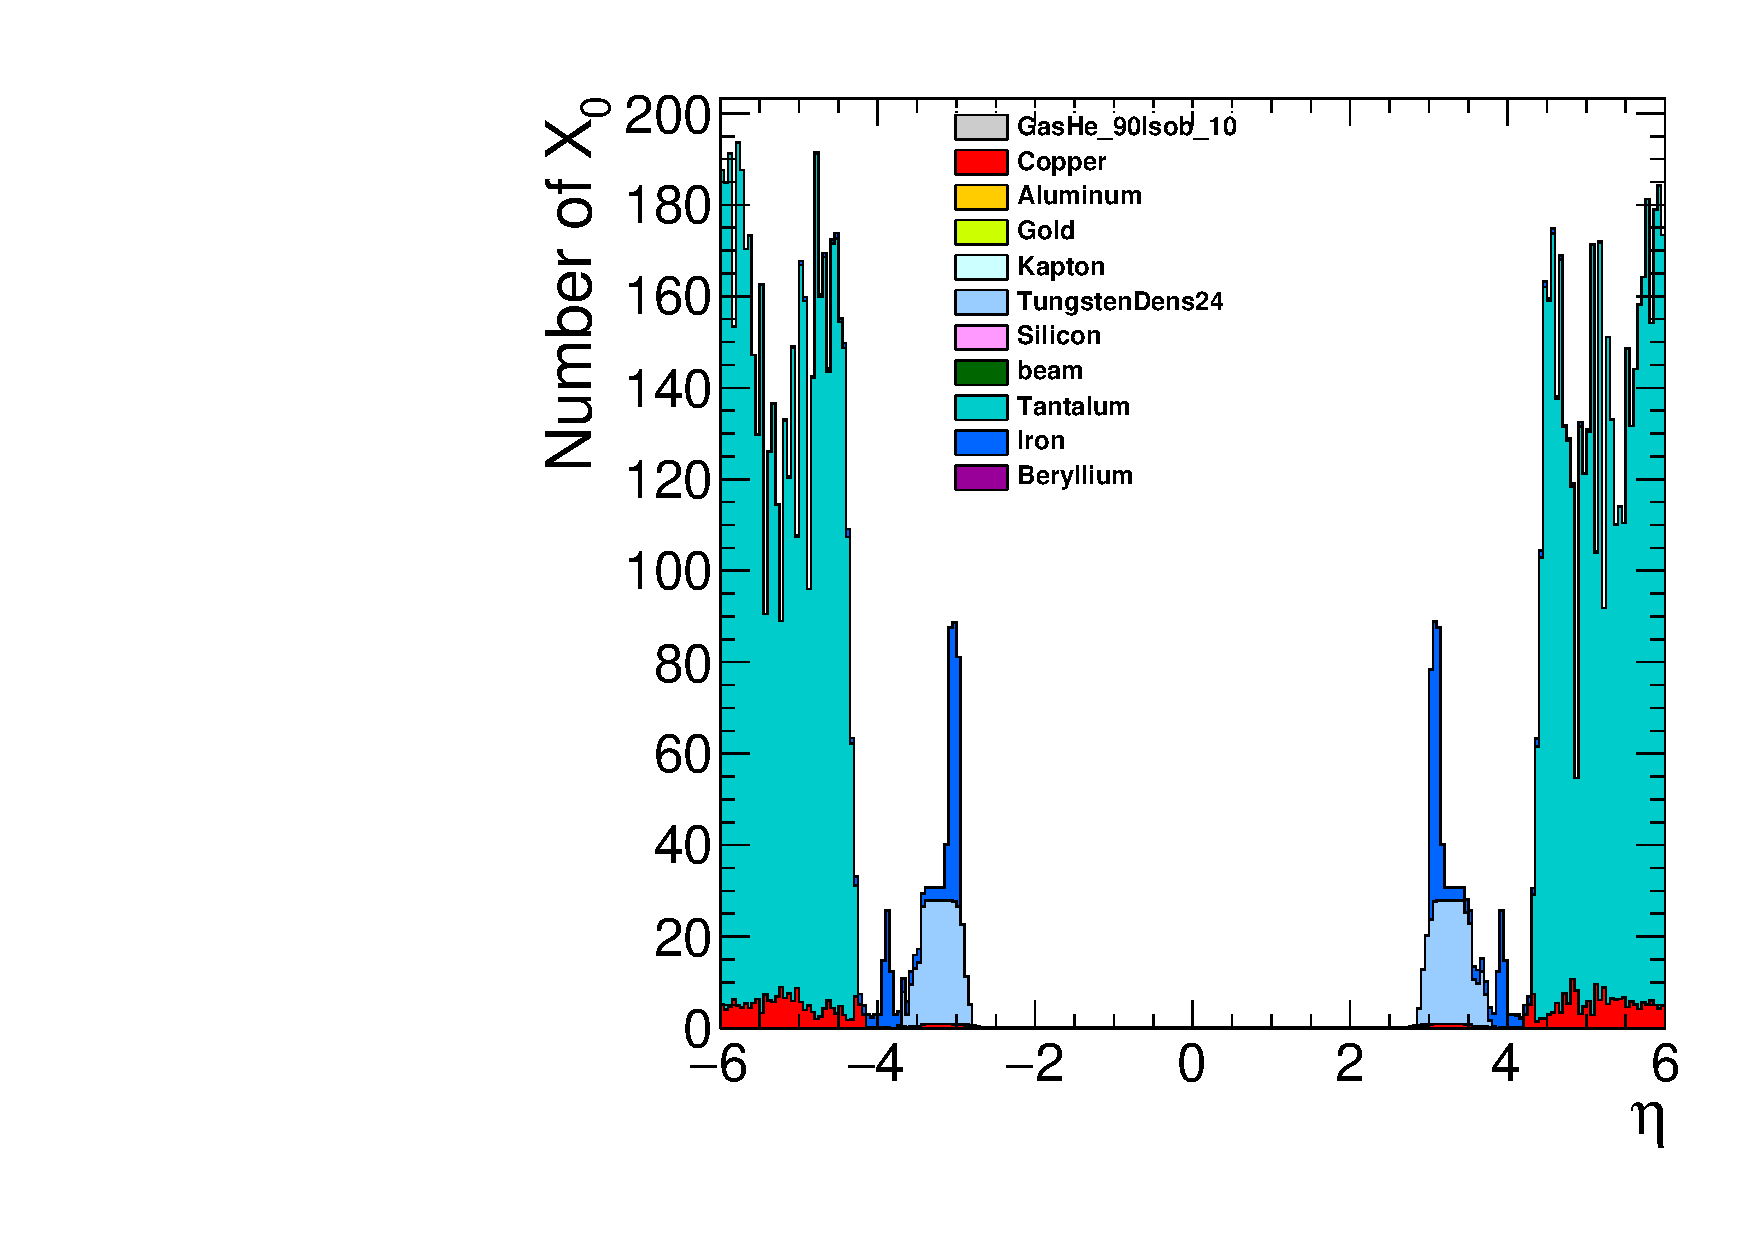
\includegraphics[width=\textwidth]{../figures/material/x0.pdf}\\
%	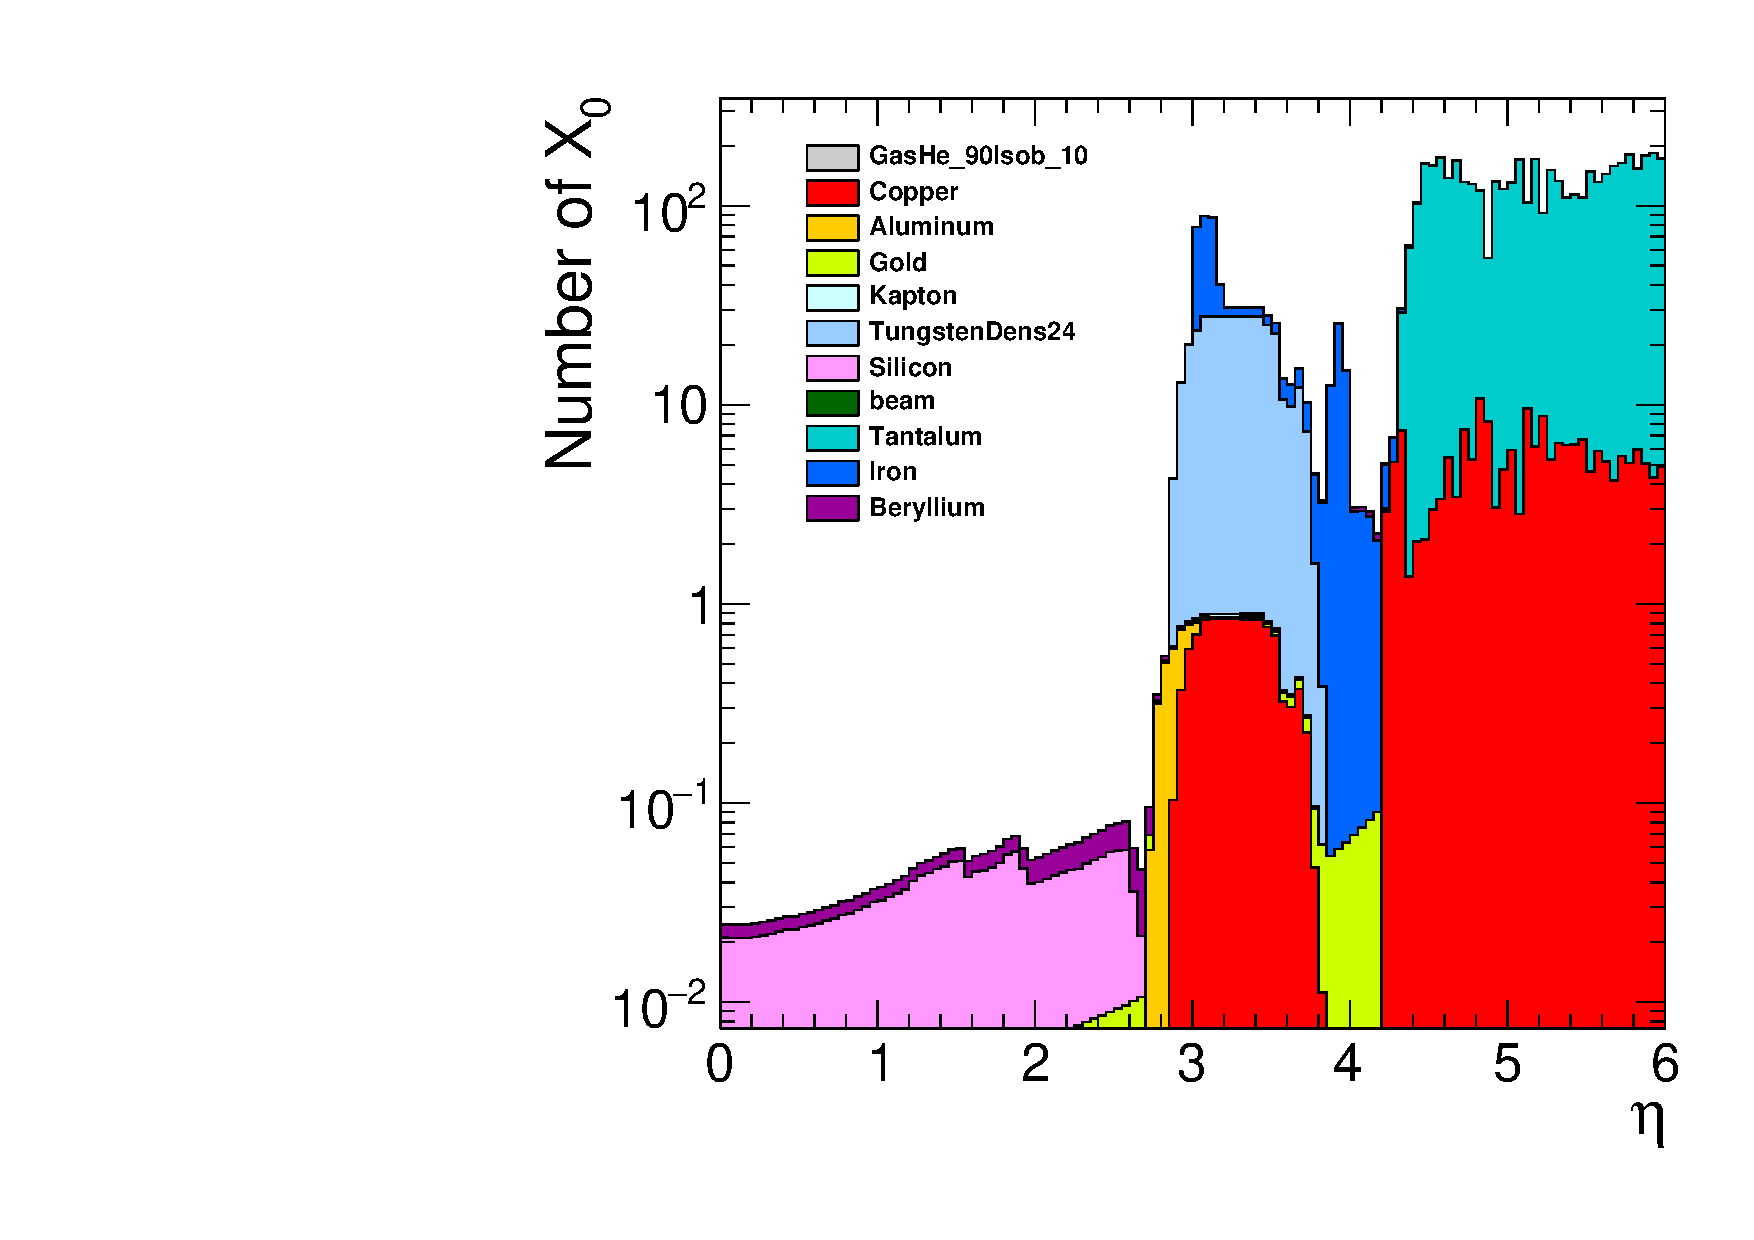
\includegraphics[width=\textwidth]{../figures/material/x0pos.pdf}
%  \end{columns}
%
%\end{frame}
%----------------------------------------------------------------------------------------
%	End of Document
%----------------------------------------------------------------------------------------
\end{document} 
